\documentclass[11pt,twocolumn]{article}
\usepackage[a4paper,margin=0.50in,columnsep=0.25in]{geometry}
\usepackage{amsmath,amssymb,booktabs,graphicx,array}
\usepackage[hidelinks]{hyperref}
\usepackage{xurl}
\hypersetup{pdftitle={ARX--RBF Motion Modeling for Cyberattack Detection and Recovery Monitoring in Industrial Robots},pdfauthor={Muhammad Usman; Haiqa Mushtaq; Muhammad Inaam ul Haq; Muhammad Bilal Zahoor}}
\DeclareMathSizes{10}{10}{8}{6}
% Use cached class resources with a 10/10.5pt body and compact journal headings.
\makeatletter
\renewcommand{\normalsize}{\@setfontsize\normalsize{10}{10.5}\abovedisplayskip 8pt plus 2pt minus 3pt\belowdisplayskip 8pt plus 2pt minus 3pt\abovedisplayshortskip 0pt plus 3pt\belowdisplayshortskip 5pt plus 3pt minus 3pt}
\renewcommand\section{\@startsection{section}{1}{\z@}{-2.5ex plus -1ex minus -.2ex}{1.2ex plus .2ex}{\normalfont\large\bfseries\raggedright}}
\renewcommand\subsection{\@startsection{subsection}{2}{\z@}{-2ex plus -.5ex minus -.2ex}{.8ex plus .2ex}{\normalfont\normalsize\bfseries\raggedright}}
\renewcommand\subsubsection{\@startsection{subsubsection}{3}{\z@}{-1.8ex plus -.5ex minus -.2ex}{.6ex plus .2ex}{\normalfont\normalsize\itshape\raggedright}}
\makeatother
\setlength{\emergencystretch}{2em}
\raggedbottom
\setlength{\textfloatsep}{11pt plus 2pt minus 2pt}
\setlength{\dbltextfloatsep}{12pt plus 2pt minus 2pt}
\setlength{\floatsep}{10pt plus 2pt minus 2pt}
\renewcommand{\topfraction}{0.9}
\renewcommand{\dbltopfraction}{0.9}
\setcounter{dbltopnumber}{4}\setcounter{totalnumber}{6}
\renewcommand{\textfraction}{0.07}
\renewcommand{\floatpagefraction}{0.8}
\renewcommand{\dblfloatpagefraction}{0.8}
\newtheorem{proposition}{Proposition}
\newenvironment{proof}{\par\noindent\textit{Proof.}\ }{\hfill\textit{Q.E.D.}\par}
\title{ARX--RBF Motion Modeling for Cyberattack Detection and Recovery Monitoring in Industrial Robots}
\author{%
\normalsize Muhammad Usman\textsuperscript{1}\quad Haiqa Mushtaq\textsuperscript{1}\\[3pt]
\normalsize Muhammad Inaam ul Haq\textsuperscript{1}\quad Muhammad Bilal Zahoor\textsuperscript{2}\\[6pt]
\small \textsuperscript{1}Department of Computer Science\\
\small COMSATS University Islamabad, Sahiwal Campus\\
\small Sahiwal, Pakistan\\[3pt]
\small \textsuperscript{2}Independent researcher\\
\small Lahore, Pakistan\\[5pt]
\small Muhammad Usman: \href{mailto:me@usman.ee}{\nolinkurl{me@usman.ee}}\\
\small Haiqa Mushtaq: \href{mailto:haiqamushtaq20@gmail.com}{\nolinkurl{haiqamushtaq20@gmail.com}}\\
\small Muhammad Inaam ul Haq: \href{mailto:minaamulhaq@cuisahiwal.edu.pk}{\nolinkurl{minaamulhaq@cuisahiwal.edu.pk}}\\
\small Muhammad Bilal Zahoor: \href{mailto:Bilbzzah@gmail.com}{\nolinkurl{Bilbzzah@gmail.com}}}
\date{}
\begin{document}
\makeatletter
\twocolumn[\begin{@twocolumnfalse}
\vspace{-12pt}\maketitle\vspace{-12pt}
\begin{abstract}
A robot can remain displaced after an unauthorized command ends. A predictor that follows measurements may lose evidence of that displacement; an inaccurate protected reference may instead prolong an alarm after return. We examine command-driven motion references, nonlinear correction and recovery decisions under model mismatch. An initial frozen audit evaluates 17 controls on 189 synthetic episodes: RBF correction reduces benign alarm points by 2.01\%, below its declared 10\% target. A matched replay attributes most of the occupancy effect to alarm persistence. A second frozen campaign evaluates 11 methods on 216 new simulation episodes. A contextual envelope reduces benign alarms but fails its composite criterion because fresh-detection delay and inactivity during physical deviation increase. A transferred recurrent detector then detects only 9 of 24 interventions on an exposed simulation grid. Exact score decomposition shows task- and channel-dependent prediction-error and variance changes, rather than universal error absorption. We investigate a causal observation correction with hard gain and amplitude bounds, explicitly accounting for established residual-separation theory and ordinary linear controls. In a prospectively frozen 33-method normal-only feasibility test, the selected adapter reduces RMSE by 11.06\% but worsens an empirical sufficient-radius proxy by 8.37\% against the direct reference; a matched linear filter is also more accurate. The candidate therefore fails its advancement criterion. Retained outcomes, common-information controls and verified saved artifacts distinguish improved prediction from useful detection evidence. The investigation does not establish an original superior detector or real-robot recovery performance.
\end{abstract}
\noindent\textbf{Keywords:} digital twins; industrial robots; anomaly detection; recovery monitoring; system identification; model mismatch.
\vspace{12pt}
\end{@twocolumnfalse}]
\makeatother
\section{Introduction}

An industrial robot does not necessarily return to its intended trajectory when an unauthorized command stops. Its position and velocity reflect the earlier disturbance, the controller's response and the plant dynamics. An alarm that clears as soon as prediction error falls can therefore disappear while the robot is still displaced. The opposite error is also possible: the robot returns, but an inaccurate reference keeps the alarm active. These two failures concern the meaning of the reference as much as the accuracy of the detector.

Digital twins provide a useful setting for studying this problem because they connect observations with a representation of the physical process. Recent surveys cover their roles in security monitoring and infrastructure lifecycle security~\cite{securitysurvey,lifecycle}. Those roles require more than a low forecasting error. A reference must represent the behavior relevant to the decision. For an attack alarm, that may be the motion the robot would have followed under approved commands, rather than the next motion most consistent with recent measurements.

Robotic anomaly detectors such as CASPER and its edge-computing successor learn regularities in external motion sensing~\cite{casper,edge}. Hybrid robot twins also combine mechanical, control and learned components~\cite{hybrid}. These approaches motivate prediction-based monitoring, but they do not make all prediction residuals interchangeable. An observation-following predictor may become accurate during a sustained unauthorized trajectory. A command-driven reference can retain the discrepancy, provided its clean initialization and approved-command history remain trustworthy. Its accuracy under legitimate changes then becomes central to false alarms and clearance.

We ask: \emph{when does a command-driven motion reference retain useful evidence of sustained deviation and support alarm clearance under model mismatch?} The study assumes a protected copy of approved commands and noisy but honest joint measurements. It tests an explicit candidate: a stable autoregressive reference with a frozen radial-basis correction, followed by short- and long-window return checks. The correction is fitted on clean commissioning data; it cannot learn from an attack during monitoring. This choice makes the information boundary inspectable, but does not establish either algorithmic novelty or physical safety.

The original investigation proceeds through five linked validation studies. An initial recovery experiment motivates a clean-data identification study; a separate inertial-sensing study checks predictor training under common inputs; a residual experiment isolates uncertainty in windowed return evidence; and a frozen candidate audit measures detection, false alarms, recovery and component effects together. Later designs use earlier outcomes as development evidence. They do not retroactively become independent confirmations of the earlier hypothesis. This distinction follows the broader need to separate model selection from security evaluation~\cite{arp}. Subsequent chronological cross-validation and author-code forecasting runs extend normal-prediction assessment. A matched-control replay then diagnoses the alarm mechanism, and a separate frozen campaign tests a bounded contextual-envelope replacement on new simulation conditions. A transferred recurrent detector and a no-fit score decomposition further distinguish observation prediction from sustained-deviation evidence. This motivates a final, explicitly normal-only feasibility test of gain-limited observation correction against matched ordinary controls.

The comparisons jointly assess normal prediction, sustained attack evidence and clearance cost. Matched component removals distinguish reference accuracy from alarm persistence; a single $F_1$ value cannot resolve these effects.

The supported findings are as follows. First, we specify and test a command-driven reference and alarm-state model with an explicit separation between observed residuals and evaluator-only physical return. Second, matched controls and ablations show that protected reference evolution, nonlinear correction and alarm persistence have different effects: the simpler reference retains the main benefit, while the proposed correction fails its improvement criterion. Third, a separately frozen contextual-envelope investigation demonstrates that reducing benign alarms can preserve an advantage over matched hysteresis while still violating delay and physical-support constraints against a simple reference. Commissioning and uncertainty diagnostics help interpret these outcomes. Finally, a complete constrained observation-correction candidate is tested against command-only, constrained linear, saturation and Kalman controls under one normal-data contract. Its prediction gain does not survive the declared sensitivity/error criterion. These are empirical and methodological findings; the lower-bound algebra has established antecedents, and the present evidence does not validate a new state-of-the-art detector.




\section{Literature Review}\label{sec:literature}

\subsection{Robot monitoring and reference identification}
CASPER couples external inertial sensing with context-aware industrial-arm anomaly detection~\cite{casper}. The subsequent edge study develops real-time processing for related robotic monitoring~\cite{edge}. Their sensing modality differs from the joint positions, velocities and protected commands used here. We therefore examine independently implemented CNN predictors on a common nominal inertial recording in a separate track. An error measured in that track cannot be interpreted as attack-detection superiority over either complete published system.

Ayankoso et al. combine robot mechanics, drives, control and learned uncertainty accommodation in a hybrid condition-monitoring twin~\cite{hybrid}. Data-driven robot calibration is itself a broad research area~\cite{calibration}; adding a learned correction to a nominal reference is not sufficient evidence of novelty. Classens et al. address structured mechanical-system identification using instrumental variables and block-coordinate descent~\cite{identification}. Our finite autoregressive search uses ordinary least-squares regularization and tests an application-specific recovery requirement, rather than extending that identification theory.

The voraus-AD study provides real robot executions and MVT-Flow, a normalizing-flow anomaly detector~\cite{voraus}. It is a relevant public comparator for an independent real-robot track because both data and author code can be inspected. Its published full-execution likelihood is an offline episode score. Comparing it directly with an online alarm-clearance delay would change the task. FactoryNet extends public industrial data coverage and exposes setpoints, effort, feedback and context in a common schema~\cite{factory}. Its latest manuscript is a preprint, and its releases combine new acquisitions with repackaged sources. Independence must be assessed by acquisition, not by dataset name.

\subsection{Forecasting, uncertainty and runtime decisions}
ModernTCN examines convolutional time-series modeling~\cite{moderntcn}, iTransformer attends across variates for forecasting~\cite{itransformer}, and TimeMixer uses decomposable multiscale mixing~\cite{timemixer}. We execute their author model code on the common normal IMU prediction task. Their published forecasting benchmarks differ from robotic attack detection, so this transfer evaluates prediction under our declared inputs and budget. A more accurate predictor of corrupted motion can still be less useful for retaining attack evidence.

Interval-observer fault detection already treats model uncertainty and observer design explicitly~\cite{interval}. FAIL-Detect calibrates uncertainty-aware runtime failure monitors from successful robot rollouts~\cite{fail}. We include a constant episode-band control inspired by that calibration principle in the earlier experiment, without claiming to reproduce its policy-specific signal construction or full method. Howard et al. develop time-uniform confidence sequences~\cite{howard}; our Gaussian window diagnostic uses simpler tail bounds and error spending under stated assumptions.

Kaisar et al. combine a kinematic twin, supervisory handover and consistency-gated recovery~\cite{kaisar}. We inspected their publicly accessible accepted author manuscript, not a verified final publisher PDF. Their Eq.\ 31 averages exponential squared-distance agreement between EKF and kinematic position estimates. Table 4 requires cleared alarm severity, observer agreement and minimum rescue duration for RESCUE-to-HANDOVER. Its direct RESCUE-to-NOMINAL guard lists cleared severity, observer agreement and a small path-error proxy for consecutive steps; a minimum rescue duration is not separately listed for that transition. Algorithm 1 synchronizes the kinematic estimate to the EKF in NOMINAL and resets it to the last trusted state on RESCUE entry. Its measurement decoupling is therefore mode-specific. Our reference stays decoupled after initialization, but this difference in a downstream-command attack task does not establish a new recovery principle or superiority over their pose-sensor attack/controller architecture. RESCUE uses counterfactual interventions to evaluate the usefulness of runtime alarms~\cite{rescue}. Our counterfactual serves a narrower purpose: measuring when a simulated plant returns to the trajectory it would have followed without command corruption.

Input-dependent residual thresholds already compensate for model uncertainty~\cite{inputthreshold}. Schubert et al. predict maneuver-dependent motion-control error and compare conformalized bounds with available lateral margin~\cite{motionconformal}. These precedents constrain any claim based on command context, nominal-error intervals or comparison with a physical tolerance. Our empirical envelopes cannot inherit their assumptions or coverage guarantees.

Evaluation also matters. TSB-AD examines the reliability of time-series anomaly-detection comparisons~\cite{tsbad}, while VUS studies accuracy measures for temporal anomalies~\cite{vus}. We retain unadjusted point metrics and separately report event detection and recovery. We do not adopt point adjustment or optimize a threshold on test attacks.

\subsection{Limitations and unresolved comparison requirements}
The literature supports the individual ingredients of prediction, correction, uncertainty calibration and persistent alarm state. It does not justify treating their combination here as automatically new. The principal comparison gaps are specific: different sensing modalities for CASPER, a full-execution objective for MVT-Flow, unresolved implementation correspondence for some published systems, and missing physical-return labels in public fault data. These are limits on what our experiment can establish, not evidence that the cited systems are generally defective. A claim of superiority requires a compatible implementation and matched information access.


\section{Methods}\label{sec:methods}
\subsection{State, information and threat model}
Let $x_t=(q_1,q_2,\dot q_1,\dot q_2)$ be the physical state and $x_t^0$ the state of the same plant under the complete approved command history without corruption. The monitor observes $y_t=x_t+n_t$ and approved position/velocity commands $u_t$. Its maintained state comprises predicted-state and command histories, residual buffers, an alarm bit and a return counter. The evaluator alone receives $x_t$, $x_t^0$ and the corruption schedule. Figure~\ref{fig:model} shows this information boundary.

The attacker changes commands delivered downstream of a protected command copy. Clean commissioning data, the first 100 initialization observations and that copy are trusted. Measurements contain noise, but adversarial sensor forgery is outside this experiment. Once initialized, the protected reference consumes no new measured state. This prevents corrupted motion from changing its predicted history or fitted parameters. It is conditional on the protected inputs, and does not address compromise of both commands and telemetry.

The reference estimates the response to approved commands, initialized from the clean prefix and synchronized through command timing. It is an empirical motion reference, without online parameter adaptation or validated industrial physical fidelity.

\begin{figure*}[t]
\centering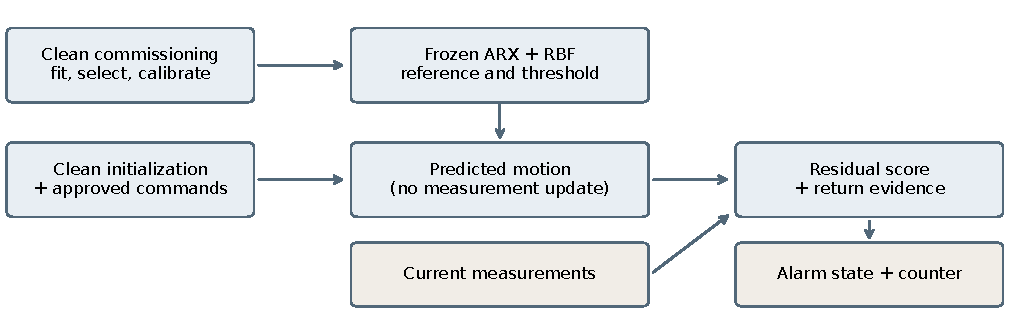
\includegraphics[width=0.82\textwidth]{figures/model.pdf}
\caption{Tested reference and alarm model. Clean data determine the frozen recurrence, correction and threshold. Approved commands drive the reference after initialization. Measurements determine residuals and alarm state, without updating the reference. Counterfactual physical return is restricted to evaluation.}\label{fig:model}
\end{figure*}

\subsection{Stable command-driven reference}
The base is a clean-data autoregressive model with exogenous inputs (ARX). In its fitted coordinates,
\begin{align}
 b_t&=a+\sum_{k=1}^{p}A_k b_{t-k}+\sum_{k=1}^{p}B_k u_{t-k},\label{eq:base}\\
 r_t^0&=\mu+s\odot b_t .
\end{align}
Commands retain their recorded physical coordinates. Training supplies state location $\mu$ and positive scales $s$; constant or nonfinite state channels are rejected. After initialization, Equation~\ref{eq:base} uses predicted states in its own history. The plant-specific orders are 8, 16 and 32 for Q1--Q3, and each selected companion matrix has spectral radius below one. Stability concerns this fitted linear recurrence; it does not establish bounded physical error under arbitrary commands or guarantee transfer to a different robot.

The following control instead uses measured history to predict the next observation. This changes the reference target while retaining the available channels.

\subsection{Training-only residual correction}
A correction estimates systematic normal residuals without feeding them back into the ARX recurrence. Its feature vector is
\begin{align}
 f_t&=[r_t^0,u_{t-1},u_{t-4},u_{t-16},u_{t-32}],\\
 z_t&=(f_t-\mu_f)/s_f,\label{eq:features}
\end{align}
with 20 dimensions. The feature means and scales use training observations only; a feature scale at or below $10^{-12}$ is replaced by one. This is distinct from rejecting a constant physical-state scale. Farthest-point selection in standardized training space deterministically chooses $K$ centers $c_i$, starting from the observation closest to the origin. The bandwidth $h$ equals a selected multiplier times the median positive center distance.

The radial basis functions (RBFs) and corrected output are
\begin{align}
 \phi_i(z)&=\exp\{-\|z-c_i\|_2^2/(2h^2)\},\\
 r_t&=r_t^0+s\odot W^T[\phi_1(z_t),\ldots,\phi_K(z_t),1]^T.\label{eq:rbf}
\end{align}
The four-output coefficient matrix minimizes
\begin{equation}
 N^{-1}\|\Phi W-E\|_F^2+\lambda\|W_{1:K,:}\|_F^2,\label{eq:fit}
\end{equation}
where $E$ contains standardized clean residuals. The intercept is unpenalized, and nonfinite fits are rejected. A linear correction uses the same 20 standardized features and objective, providing a direct nonlinearity control. RBF heads contain $4(K+1)$ coefficients: 132 for 32 centers and 260 for 64 centers. These counts exclude stored centers, feature statistics and the base ARX. The linear head contains 84 coefficients.

Bounded activations and fixed weights bound correction magnitude, not physical prediction error. Weights, centers, scales and thresholds remain frozen during evaluation.

\subsection{Entry score and alarm-clearance state}
Define $e_t=(y_t-r_t)/s$ and $a_t=\max_j|e_{t,j}|$. Strict exceedance $a_t>\tau$ raises an alarm and resets its return counter. At other eligible points, the candidate checks
\begin{equation}
 g_t=\mathrm I\!\left\{\|\bar e_t(5)\|_\infty\le0.1\ \land\
 \|\bar e_t(41)\|_\infty\le0.1\right\},\label{eq:gate}
\end{equation}
where $\bar e_t(m)=m^{-1}\sum_{k=0}^{m-1}e_{t-k}$. Ten consecutive qualifying points clear an active alarm; a new entry exceedance has priority. The windows contain 0.10 and 0.82 seconds of samples at 50 Hz, and the dwell contains 0.20 seconds. Entry scoring starts at zero-based index 100 and covers 1,100 points per episode. Clearance uses only residuals from that scored interval: the five-point window first becomes ready at index 104 and the 41-point window at 140. Dual-window clearance can first occur at 149 with ten-point dwell, or at 140 without dwell. Entry remains possible before clearance readiness; these distinct eligibility masks do not shorten the score population. Signed means can cancel oscillatory deviations, so the gate measures agreement with the reference rather than certifying physical return.

The short gate is partly constrained by the entry rule: after five consecutive non-exceedances, the mean residual norm is no greater than the largest of those five scores, hence no greater than $\tau$. The RBF thresholds are 0.03697, 0.03712 and 0.05740, all below 0.1. Thus the short gate passes on those windows. Earlier exceedances can still alter streak timing; this conditional result is not a universal equivalence proof.

Invalid history resets the evidence streak and cannot clear an active alarm; the implemented known-state mask then remains false. The final campaign admits complete finite episodes, so missing-data behavior is software-tested only. Algorithm~\ref{alg:replay} specifies the causal order.

\begin{table*}[t]\centering
\caption{Algorithm 1: normal-only fitting, selection and freezing.}
\label{alg:fit}
\begin{tabular}{>{\raggedright\arraybackslash}p{0.055\textwidth}>{\raggedright\arraybackslash}p{0.88\textwidth}}\toprule
Input & Separate clean training, development and calibration episodes; declared candidate grid and tie-break rule.\\\midrule
1 & Fit training-only state statistics and candidate ARX references; reject invalid or unstable candidates. Preserve each candidate outcome.\\
2 & Generate free-running training predictions from clean initial histories. Construct the 20-dimensional features and fit their statistics and centers on training only.\\
3 & Solve the ridge objectives. Evaluate each frozen candidate on the same normal-development episodes, keeping episode boundaries intact.\\
4 & Within the linear and RBF roles separately, select by worst-episode residual $q_{.99}$, then mean RMSE, coefficient count and identifier. Preserve the chosen artifact without refitting on development.\\
5 & Score the separate normal-calibration population. Set the fixed entry threshold to ascending rank 5,445 of 5,500 scores.\\
6 & Seal models, transforms, thresholds, methods, seeds, inputs, code, budgets and criteria before generating the new evaluation conditions.\\\bottomrule
\end{tabular}
\end{table*}

\begin{table}[t]\centering
\caption{Algorithm 2: prospective monitoring of one episode.}\label{alg:replay}
\begin{tabular}{>{\raggedright\arraybackslash}p{0.12\columnwidth}>{\raggedright\arraybackslash}p{0.76\columnwidth}}\toprule
Input & Frozen model and threshold; clean 100-point prefix; approved commands and current measurements.\\\midrule
1 & Initialize predicted history from the prefix; set alarm, evidence counter and post-prefix residual buffers to zero/empty.\\
2 & Predict $b_t$ from earlier predicted states and commands; compute $r_t$ using the frozen correction.\\
3 & At $t\ge100$, read $y_t$, score and append $e_t$. Before full post-prefix windows exist, entry is allowed but clearance is not. No label or future measurement is read.\\
4 & If history is invalid, reset the streak and retain alarm state. Otherwise, an entry exceedance raises alarm and resets the streak.\\
5 & If alarm is active without an exceedance, increment the streak when $g_t=1$, otherwise reset it. Clear after the declared dwell.\\
6 & Save score, validity and alarm at index $t$. Advance predicted history, leaving fitted parameters fixed. Continue across attack boundaries.\\\bottomrule
\end{tabular}
\end{table}

\subsection{Physical return and uncertainty}
The evaluator measures $d_t=\max_j|x_{t,j}-x_{t,j}^0|/s_j$. Reference/noise bounds $b_t,\eta_t$ would give $d_t\le a_t+b_t+\eta_t$. Sufficient return requires $a_t+b_t+\eta_t\le\delta$, which is infeasible when the allowance exceeds the tolerance. Empirical maxima under Gaussian noise are not deterministic bounds. Appendix~\ref{app:uncertainty} develops this limitation and the window diagnostic.
\subsection{Bounded extension: contextual residual evidence}\label{sec:contextmethod}
The matched replay diagnoses excessive retention of noisy entries, with a smaller concentration of errors around legitimate command steps. We therefore investigate a command-conditioned empirical allowance using the saved base ARX; RBF is not required by this extension. The context state depends only on approved command increments:
\begin{align}
 d^u_t&=\|(u_t-u_{t-1})/s\|_\infty,\\
 h_t&=\max\{d^u_t,\exp(-1/m)h_{t-1}\},\quad h_0=0.
\end{align}
Training 90th/99th context quantiles define three bins. Each bin's width $w_t$ is the ascending 99th-percentile base residual score on separate normal calibration observations, with a global-quantile fallback below 30 observations. Context state evolves causally, but bin boundaries, widths and reference parameters are frozen. The top bin extends beyond the training maximum: this is empirical extrapolation, with context-support frequency reported, not a guaranteed uncertainty set.

Using the instantaneous residual score $a_t$, define
\begin{equation}
 L_t=\max(0,a_t-w_t),\qquad U_t=a_t+w_t.
\end{equation}
The candidate enters when $L_t>0.1$, clears when $U_t\le0.1$, and otherwise retains its previous state. No dwell or residual averaging is added. The unresolved region is reported even when the alarm is inactive. If $w_t$ truly bounded the combined nominal-reference and measurement error in the same standardized infinity norm, triangle inequalities would give $L_t\le d_t\le U_t$. An empirical normal quantile does not establish that bound under attack or plant shift. We test the decision rule as a heuristic, without a coverage or safety theorem.

The finite candidate set uses memories $m=10,40$ samples (0.2/0.8 s). K13 normal episodes fit bin boundaries; L13 normal episodes calibrate widths; M13 normal episodes select by benign alarm points, starts, mean allowance and then memory. These are exposed development data separated by task, not fresh validation. Two memories on each plant give six plant-specific fits across two candidate memory choices; no ARX or RBF weights are refitted. The selected candidate is frozen before new evaluation.

The essential matched control uses identical context and entry decisions but clears at $a_t\le0.1$, isolating the extra width in clearance. Other controls use a constant global width, contextual entry without retention, the physical-tolerance point rule $a_t>0.1$, and a three-of-five original-threshold entry rule, alongside the historical base/RBF and following rules. Input-dependent thresholds, residual intervals and hysteresis already exist~\cite{inputthreshold,motionconformal,interval}; an observed gain would require a specific advantage over these ordinary controls before an originality argument.



\section{Experiments}\label{sec:experiments}
\subsection{Datasets and experimental populations}
The study separates simulated attack/recovery evaluation, real-data normal prediction and admission of future public evidence (Table~\ref{tab:data}). They answer different questions and are not pooled into one performance ranking. Five linked studies document the development sequence: E1 recovery, E2 commissioning, E3 nominal IMU prediction, E4 residual uncertainty and E5 original RBF evaluation. Later choices use earlier outcomes as development; the earlier studies do not become independent confirmations of those choices.

\begin{table*}[t]\centering
\caption{Data and information boundaries. Counts identify the populations actually used or admitted. New public-data receipt is not an additional experiment.}\label{tab:data}
\begin{tabular}{>{\raggedright\arraybackslash}p{0.18\textwidth}>{\raggedright\arraybackslash}p{0.23\textwidth}>{\raggedright\arraybackslash}p{0.26\textwidth}>{\raggedright\arraybackslash}p{0.23\textwidth}}\toprule
Source & Population & Permitted model information & Status and interpretation\\\midrule
Two-joint simulation, E5 & 3 training, 9 development and 5 calibration episodes per plant; 81 fresh normal and 189 audit episodes & Noisy joint position/velocity and protected approved commands; clean initialization & Synthetic, with evaluator-only command intervals and same-plant physical-return truth.\\
CASPER provider-v2 nominal IMU, E3 & 8,192 common training and 2,048 development targets; nine channels & Past causally filtered accelerometer, gyroscope and magnetometer observations & Real nominal prediction; no attack evaluation, unresolved paper-release and clock correspondence.\\
voraus-AD original 100 Hz release & 2,122 executions; original split 948 training / 1,174 test & No process signals admitted to modeling yet & Metadata verified only; normal/fault labels, no established cyber or physical-return labels.\\
FactoryNet & Author-reported mixed real/synthetic corpus & No observations downloaded & Partially admitted source; imported sources are not new independent acquisitions.\\\bottomrule
\end{tabular}
\end{table*}

\subsubsection{Physical simulator and command construction}
The plant is a horizontal two-joint point-mass arm:
\begin{equation}
 M(q)\ddot q+C(q,\dot q)+B\dot q=\tau.\label{eq:plant}
\end{equation}
For $a=m_2l_1l_2$ and $d=m_2l_2^2$, its inertia entries are $M_{11}=(m_1+m_2)l_1^2+d+2a\cos q_2$, $M_{12}=M_{21}=d+a\cos q_2$, and $M_{22}=d$. The Coriolis vector is $a\sin q_2[-2\dot q_1\dot q_2-\dot q_2^2,\dot q_1^2]^T$. A proportional--derivative controller requests
\begin{equation}
 \tau^*=\operatorname{clip}\{K_p(q^c-q)+K_d(\dot q^c-\dot q),-20,20\},
\end{equation}
with diagonal gains $(18,12)$ and $(4,3)$. With actuator lag, $\dot\tau=(\tau^*-\tau)/T_a$. Nominal masses are $(1,0.8)$ kg, lengths $(0.5,0.4)$ m and damping $(0.08,0.06)$; Table~\ref{tab:plants} defines the actual plants. Position and velocity noise are independent zero-mean Gaussian with standard deviations 0.0005 rad and 0.002 rad/s before the plant multiplier.

\begin{table*}[t]\centering
\caption{Fixed simulated plants. Mass and damping factors multiply the nominal values; noise multiplies both sensor standard deviations.}\label{tab:plants}
\begin{tabular}{lcccrr}\toprule
Plant & Mass factors & Damping factors & Lengths (m) & Lag (s) & Noise\\\midrule
Q1 & (1.10,0.86) & (0.80,1.20) & (0.48,0.42) & 0 & 1.0\\
Q2 & (0.88,1.15) & (1.30,0.85) & (0.53,0.37) & 0.03 & 1.0\\
Q3 & (1.16,1.06) & (0.90,1.40) & (0.46,0.43) & 0.06 & 1.5\\\bottomrule
\end{tabular}
\end{table*}

Sampling is 50 Hz with eight fourth-order Runge--Kutta substeps per sample. A separate short integration check supports numerical consistency, not fidelity to an industrial robot. Gravity, contact, flexibility and thermal effects are absent. Approved positions are
\begin{align}
 q_1^c&=a_1\sin\theta+0.025\sin(2.3\theta),\\
 q_2^c&=a_2\sin(\theta+\phi)+0.018\sin(1.7\theta),
\end{align}
with analytic velocities under the causal time warp. The final tasks are N14: $\theta=0.49t$, amplitudes $(0.28,0.37)$, phase 0.93; O14: $\theta=0.43t+0.008t^2$, amplitudes $(0.33,0.31)$, phase 0.72; and P14: $\theta=0.94t+0.18\sin(0.31t)$, amplitudes $(0.35,0.38)$, phase 1.14.

The final audit crosses these three tasks, three existing plants, seeds 17, 42 and 2026, and seven conditions: ordinary operation, authorized offset, authorized slowdown, brief unauthorized offset, persistent offset, hold and slowdown. There are 81 wholly benign and 108 attack episodes. Each contains 1,200 samples, including the clean 100-point initialization. Corruption begins at index 347 and ends before 653, except the eight-point brief offset. Offset magnitude is 0.11 rad on joint 1; slowdown rate is 0.72. An offset adds 0.11 rad only to the first position command during the half-open intervention interval; recorded velocity commands are unchanged, so the boundary is a commanded step. Hold fixes both positions to their index-346 values and sets both commanded velocities to zero until index 653. Slowdown uses $v_t=0.72$ within the interval and one elsewhere, causal warped time $s_t=0.02\sum_{j<t}v_j$, and the analytic derivative of the trajectory at $s_t$ multiplied by $v_t$. Unauthorized slowdown restores the original unwarped command at index 653; authorized slowdown retains its accumulated phase lag. Authorized changes update the protected command copy, while attacks change only delivered commands. Truth and schedule remain outside inference.

\subsubsection{Real nominal recording and independent sources}
The separate IMU study uses the provider-v2 nominal \texttt{IMU\_10Hz.csv}, with accelerometer, gyroscope and magnetometer axes. It differs from the original CASPER-v3 archive. Exact correspondence to the published runs, timestamp units and acquisition-versus-arrival timing remain unresolved. We report sample-based prediction errors, not physical-time attack delays inferred from the filename.

voraus-AD metadata and original splits were verified, but its process signals remain unopened~\cite{voraus}. FactoryNet remains source-audited only~\cite{factory}. Appendix~\ref{app:provenance} records hashes, permissions, source overlap and code-admission issues; neither source contributes measured model results here.

\subsection{Preprocessing, chronology and calibration}
\subsubsection{Synthetic commissioning and held-out conditions}
Three clean commissioning episodes per plant fit the base and corrections. Their rates are 0.35, 0.7 and 1.1, with amplitudes $(0.22+0.04i,0.34-0.025i)$ and phase $0.5+0.3i$ for $i=0,1,2$, covering unchanged, authorized-offset and authorized-slowdown motion. The earlier normal episode bank uses rate $0.32+0.047i$, amplitudes $(0.23+0.012(i\bmod7),0.29+0.013(i\bmod9))$ and phase $0.4+0.06(i\bmod11)$. Indices 0--8 select configurations and 9--13 calibrate. Five remaining archived checks are not new independent data.

Transforms, centers and regression coefficients use training only. Each episode retains its own initialization and history; windows never cross episode or split boundaries. After selection, each reference has 5,500 eligible calibration scores. The ascending score at rank $\lceil0.99(5500)\rceil=5445$ fixes its threshold. Strict exceedance handles ties. Calibration cannot choose models, seeds or a better percentile. Equal point-score quantiles do not equalize a stateful rule's alarm occupancy or guarantee future 1\% false alarms.

The candidate check uses 81 new normal combinations. K13 uses $\theta=0.58t$, amplitudes $(0.30,0.36)$ and phase $1.05$; L13 uses $\theta=0.42t+0.008t^2$, $(0.32,0.35)$ and $0.95$; M13 uses $\theta=0.89t+0.18\sin(0.31t)$, $(0.29,0.39)$ and $0.65$. The attack audit freezes the fits, thresholds and 17-method roster before generating N14, O14 and P14. The tasks are new; the simulator and plants are reused. All resulting conditions are now exposed.

\subsubsection{Chronological IMU partitions}
Zero-indexed training rows $[219,9185)$ precede development rows $[9185,12007)$. Splitting occurs before the trailing width-20 median filter, training scaling and history creation. Each partition loses 19 filter warmup observations. Timestamps must increase strictly, with no gap exceeding five times the training median increment. Constant or nonfinite training channels are rejected.

All predictors share 8,192 training and 2,048 development targets after 755 history observations. Development targets are raw rows 9959--12006 inclusive. A later 755-residual aggregation has 1,294 aligned endpoints. The compact CNN uses only its 45-point history, but receives the same eligible target rows. These data were used for checkpoint selection and cannot serve as independent final evaluation.

\subsection{Experimental setup and optimization procedure}
\subsubsection{Finite model search}
The earlier reference search comprises ARX orders 4, 8, 16 and 32 and finite impulse response lengths 16, 32 and 64, crossed with ridge penalties $10^{-7},10^{-5},10^{-3}$ on each plant: 63 fits. Stable ARX orders 8, 16 and 32 with ridge $10^{-7}$ are inherited by the correction study.

The correction grid has eight RBF settings per plant: $K\in\{32,64\}$, width multiplier in $\{0.5,1\}$ and ridge in $\{0.001,0.01\}$. Two linear penalties use the same feature inputs, giving 30 fits overall. Within each correction role, selection minimizes the worst episode's 99th-percentile standardized residual, then mean episode RMSE, head coefficient count and identifier. All candidates and failures remain recorded. ``Optimal parameters'' here means selected within this finite normal-development procedure, not a global optimum or a choice based on final attacks.

\subsubsection{Neural training and stopping}
The independent CASPER-style CNN has four valid one-dimensional convolutions, each with 32 filters, kernel five and ReLU. Width-three pooling follows each pair; flattening and a nine-output dense layer give 39,977 parameters for 755-point history. The Edge-style CNN has two valid convolutions with eight filters and kernel three, width-three pooling, and a nine-output dense layer: 1,369 parameters for 45-point history. Both use zero-initialized output heads, disclosed as an implementation choice.

Adamax uses learning rate $10^{-3}$ and batches of 64 in chronological order without shuffling. A normal-development improvement greater than $10^{-6}$ selects a checkpoint; patience is five epochs and the cap is 100. Seeds 17, 42 and 2026 start afresh without optimizer transfer. Per-fit CPU admission is 240 seconds, with total limits of 1,200 seconds wall and 900 seconds CPU.

\subsubsection{Five-fold chronological validation of ARX--RBF}
After the original audit, we perform a retrospective normal-prediction check on the nine existing commissioning episodes. Each has 1,200 observations and is divided into six consecutive 200-point blocks. In fold $k\in\{1,\ldots,5\}$, training uses $[0,200k)$ in each episode. The following block supplies 100 known-normal observations for state initialization and 100 scored targets, at $[200k+100,200(k+1))$. Windows never cross a split or episode boundary. Each plant combines the training prefixes of its three episodes; all three plants therefore contribute 900 scored observations per fold.

Both the ARX control and ARX--RBF refit their means, scales, coefficients and correction features using only that fold's training prefixes. Only orders, center counts, bandwidth multipliers and ridge penalties retain the earlier settings. Center locations and numerical bandwidth are recomputed from each fold's standardized training features; they are not reused from the full-data fit. Validation measurements cannot change fitted parameters. Unstable or nonfinite fits would remain recorded as failures with zero coverage. No thresholds or attack metrics are computed. Because these settings and commissioning data were used previously, this is a developmental stability check, not nested cross-validation or independent confirmation. Expanding training prefixes overlap, and each validation trajectory has its own 100-point initialization.

\subsubsection{Recent author-code forecasting runs}
ModernTCN, iTransformer and TimeMixer use their original model classes with 96 past IMU observations and a one-step, nine-channel forecast. All receive the same 8,192 training and 2,048 development targets as E3, with its unchanged training-only scaler and causal preprocessing. Model-defined normalization uses the observed input window only; no future covariates or current target enter the predictor. The original CNNs retain their disclosed 755- and 45-point histories.

Transferred settings follow the authors' ETTh1 examples: ModernTCN has one 64-wide block, kernels 51/5, patch size eight, stride four and dropout 0.3; iTransformer has two 256-wide layers, eight heads and feed-forward width 256; TimeMixer has two layers, width 16, feed-forward width 32 and three average-downsampling levels. Adam rates are $10^{-4}$, $10^{-4}$ and $10^{-2}$ respectively. Batches of 64 follow chronological order. Each of seeds 17, 42 and 2026 starts afresh; normal-development MSE selects checkpoints with tolerance $10^{-6}$, patience five and a ceiling of 100 epochs. Each seed has a 150-second CPU admission budget, reserving the estimated cost of the next epoch. Actual stopping and coverage are reported, rather than treating a budget-limited fit as converged. Compatibility pilots allow at most two epochs and do not select hyperparameters.

\subsubsection{Execution environment and validation sequence}
Runs use macOS/arm64, Python 3.12.15 and NumPy 1.26.4; the independently implemented CNNs use TensorFlow 2.16.2. The recent author-code study uses PyTorch 2.5.1 on an Apple M5 Pro with 24 GB RAM, one Torch CPU thread and deterministic algorithms. No GPU benchmark is reported. Inference outputs are sealed before joint label evaluation. Exact execution records and failures are retained.



\subsection{Fresh evaluation of the bounded extension}\label{sec:contextstudy}
The new protocol freezes the selected envelope, inherited reference artifacts, eleven methods, conditions, seeds and success clauses before generating evaluation outcomes. Each task/plant receives identical observations and scales across methods. Historical base/RBF/following policies retain their original C9--C13 thresholds; all new envelope variants share L13 calibration. A gain against the historical policy alone therefore cannot isolate the recovery mechanism. The contextual hysteresis comparison holds the new information and entry decisions fixed. Three original plant parameterizations and three perturbations are crossed with two new task families, three seeds and six conditions, giving 216 episodes. Each perturbed plant multiplies its parent's masses by $(1.04,0.96)$, damping by $(1.10,0.90)$, and adds 0.01 s actuator lag; it receives the parent's unchanged model and calibration. This tests within-simulator transfer, not independent physical robots.

L19 commands are $(0.29\sin(0.57t),0.34\sin(1.37\,0.57t+0.77))$. S19 uses quintic reversals: $q_j^c=A_j(-1)^k[2H(v)-1]$, where $H(v)=10v^3-15v^4+6v^5$, $k=\lfloor0.14t+\phi_j\rfloor$, $v=0.14t+\phi_j-k$, $A=(0.26,0.32)$ and $\phi=(0,0.38)$. Velocity commands are analytic derivatives. Original plant integration and noise remain unchanged.

The six conditions are ordinary operation, repeated authorized offsets, brief unauthorized offset, persistent offset, hold and slowdown. Benign episodes have 6,000 samples; the 72 episodes give 424,800 eligible points (2.36 h). Authorized first-joint position offsets are $+0.07$, $-0.09$ and $+0.05$ rad on half-open index intervals $[600,900)$, $[2000,2300)$ and $[4000,4400)$. Attack episodes have 2,400 samples. L19/S19 onsets are 503/611, sustained durations 530/470, brief lengths 12/10, offsets 0.13/0.09 rad and slowdown rates 0.64/0.78. Hold/slowdown follow the earlier transformation rules. There are 144 attack episodes; state never resets at intervention boundaries.

The new prospective criterion requires at least 20\% fewer benign alarm points and 10\% fewer starts than base dual. Costs must not worsen: fresh detections cannot decrease, the fresh-detection p95 delay can increase by at most 0.2 s, outside-tolerance inactive fraction cannot increase, and the joint detected/continuously-supported/timely-inactive event count cannot decrease. The same cost constraints apply against contextual ordinary hysteresis, and the candidate must strictly improve its outside-tolerance inactivity or joint count to justify the extra recovery rule. These study-specific conditions do not define a universal acceptable industrial alarm rate. They do not replace the failed original 10\% criterion.

Unlike the earlier diagnostic's after-detection support count, the new outside-tolerance count includes all post-onset eligible points, including detection delay. The joint outcome requires an overlap hit, zero outside-tolerance inactivity and inactivity by return + 5 s with observed return. Undefined delays, misses and absent returns remain visible. Conditions are paired by task, plant and seed; rows and noise seeds are not independent robot replications. A normal-only pilot precedes final generation; doubling integration substeps changes native state by at most $4.993\times10^{-7}$. Resource admission and compact export are frozen before the single final run.



\section{Evaluation Metrics}\label{sec:metrics}
\subsection{Prediction and point-level detection}
For $N$ eligible targets and $d$ training-standardized channels, normal prediction error is
\begin{equation}
 \operatorname{MSE}=\frac{1}{Nd}\sum_{t,j}\left(\frac{y_{t,j}-r_{t,j}}{s_j}\right)^2,
 \qquad \operatorname{RMSE}=\sqrt{\operatorname{MSE}}.
\end{equation}
Development also uses the 99th percentile of $a_t=\|e_t\|_\infty$. A low normal error is not an attack-detection result. The same training scales are retained for each model's assigned evaluation.

Point counts compare the alarm bit with the command-corruption schedule on all eligible observations, without point adjustment:
\begin{align}
 P&=\frac{TP}{TP+FP},\quad R=\frac{TP}{TP+FN},\\
 F_1&=\frac{2TP}{2TP+FP+FN}.
\end{align}
Precision is zero when there are no positive predictions. Average precision (AP) uses continuous entry scores: $\mathrm{AP}=\sum_k(R_k-R_{k-1})P_k$, grouping equal scores at common thresholds. It is undefined with no positive labels. Gate variants can therefore share AP while producing different alarm trajectories. The final audit has 207,900 eligible points and 25,002 schedule-positive points per method, with complete score coverage.

\subsection{Benign alarms, event coverage and delay}
Benign occupancy is $N_{\rm alarm}/N_{\rm benign}$ on wholly benign episodes. Starts per hour divide alarm rising edges by $N_{\rm benign}\Delta t/3600$, where $\Delta t=0.02$ seconds. The final benign population is 89,100 points, or 0.495 eligible hours. Short repeated alarms and one sustained alarm may have similar occupancy but very different start rates.

An overlap hit is any alarm during an attack interval. A fresh hit requires a rising edge within that interval. Both denominators are all 108 events; a preexisting alarm can overlap without a fresh onset. Delays measure samples from schedule onset to the first qualifying overlap or rising edge, multiplied by $\Delta t$. Misses remain explicit, with undefined delays rather than silently removed or assigned zero. There is one scheduled intervention per attack episode; these are paired simulation conditions, not independent industrial incidents.

\subsection{Physical return and clearance}
Physical return is the first start of ten consecutive post-corruption states with $d_t\le0.1$. This retrospective evaluator label uses the uncorrupted same-plant trajectory and never enters inference. In native coordinates, its per-channel limits for $(q_1,q_2,\dot q_1,\dot q_2)$ are Q1 $(0.019922,0.022899,0.016145,0.015549)$, Q2 $(0.020068,0.022931,0.016379,0.015705)$ and Q3 $(0.020039,0.022972,0.016393,0.015788)$, with positions in rad and velocities in rad/s. These are declared diagnostic tolerances, not certified safety margins. The reported ``inactive by return + 5 s'' fraction counts an inactive alarm at or within 250 samples after that return, conditional on an overlap hit and an observed return. An alarm already inactive at return contributes zero delay. Consequently, 108/108 does not mean that all alarms persisted until recovery. Delay summaries retain the numbers of misses, absent returns and alarms still active at episode end; zero-delay cases are identified separately.

The registered early-clear metric records a falling edge after first overlap but before stable physical return. Gap points count inactive observations between that hit and return, or the episode end when no return exists. A continuity break near onset can count even while instantaneous deviation is small. An explicitly post-study diagnostic separately checks true deviation at early falling edges; it does not replace the registered outcome.

\subsection{Predeclared improvement and cost}
RBF dual must preserve or improve hits, fresh hits and timely clears on each plant, while not increasing early-clear events, benign alarm points or pre-return gaps. It must also reduce pooled benign points or gaps by at least 10\% relative to base dual. These are descriptive registered requirements, not statistical noninferiority tests. Secondary metrics cannot rescue a failed primary criterion.

Wall time, worker CPU, sampled resident memory and output size measure whole recorded runs. Shared computation prevents interpreting total time divided by the number of methods as per-method latency. Stochastic seeds describe computational/noise variation within the same experimental systems; no confidence interval is presented as if they were independent robot acquisitions.


\section{Comparison Methods and Baselines}\label{sec:comparators}
\subsection{Protected references and component removals}
The final roster compares base ARX, linear correction and RBF correction under matched inputs. Point rules directly threshold $a_t$. Return rules retain alarm using a one-point residual condition, the 41-point window, or the 5/41 dual window, generally with ten-point dwell. The no-dwell variant requires one qualifying point. Base long versus base dual and RBF long versus RBF dual isolate the short window; RBF dual versus its no-dwell variant isolates persistence. Base dual versus RBF dual is the primary correction comparison. Every variant keeps its declared entry score, threshold and support.

The RBF-following ablation applies the correction trained on free-running features to measured-history predictions without refitting. It tests that disclosed assembly, not an optimally fitted following model. Table~\ref{tab:audit} retains all 17 methods.

\subsection{Ordinary prediction and accumulation controls}
Persistence predicts the last measured state. The causal rolling mean predicts from the preceding 21 observations, excluding the current target. A one-sided CUSUM uses $G_t=\max(0,G_{t-1}+a_t-k)$, with $k$ equal to the training-score mean plus its standard deviation. Its calibrated statistic has no reset on alarm in this registered implementation. Its persistence is therefore a deliberate comparator behavior, not a claim that all CUSUM schemes cannot recover. All controls use identical eligible episode support and cannot access labels or truth.

The IMU controls are training mean, persistence and AR(4), alongside the CNNs specified in Section~\ref{sec:experiments}. AR fits standardized channels with ridge $10^{-3}$ on mean normal equations, leaving its intercept unpenalized. Deterministic controls run once and neural models use all three seeds.

\subsection{Recent published methods and correspondence}
The recent-paper comparison window is 16 October 2023--16 October 2026, with preference for 2024--2026. CASPER (2024) and Edge CNN (2025) are independent architectural implementations; ModernTCN, iTransformer and TimeMixer (ICLR 2024) execute author model code; MVT-Flow (IEEE T-RO 2024) remains unexecuted. Publication recency does not establish comparability or a current state-of-the-art ranking. Classical AR, persistence, rolling means and CUSUM remain explanatory controls. Older sources support observer, uncertainty and input-dependent-threshold foundations; they are not recent detector baselines.



The CNNs use independent implementations; author forecasters use unchanged model sources with our causal adapter, preprocessing and budget. These normal-development measurements are not pooled into the protected-command attack ranking. MVT-Flow remains an unexecuted offline candidate; its symmetric convolutions, whole-execution objective and source correspondence require a separate task contract. No complete published attack-detector reproduction is claimed.


\section{Results}\label{sec:results}
\subsection{Parameter selection and normal prediction}
The 63-fit E2 search selects ARX orders 8, 16 and 32 with ridge $10^{-7}$. Appendix~\ref{app:earlier} summarizes the earlier controls. For the E5 correction, all 30 candidates produce eligible outcomes. Every development criterion, including weaker settings, remains in the recorded candidate matrix. Selection chooses 32 centers on all plants, width multipliers 1, 0.5 and 1, and penalties 0.01, 0.001 and 0.001 for Q1--Q3. All selected linear penalties are 0.01. These are finite normal-development choices, not parameter choices based on the attack audit.



\begin{table*}[t]\centering
\caption{Selected E5 candidate and fresh-normal changes against the base reference. Positive error change is worse. Each selected RBF head has 132 coefficients, in addition to its stored centers and base model.}\label{tab:selection}
\begin{tabular}{lrrrrrrr}\toprule
Plant & ARX $p$ & Centers & Width & Ridge & $\tau$ & $\Delta$RMSE (\%) & $\Delta q_{.99}$ (\%) \\\midrule
Q1 & 8 & 32 & 1.0 & 0.01 & 0.036966 & +0.0050 & -0.1314 \\
Q2 & 16 & 32 & 0.5 & 0.001 & 0.037122 & -1.2205 & -1.4022 \\
Q3 & 32 & 32 & 1.0 & 0.001 & 0.057400 & -0.1002 & +0.1506 \\
\bottomrule\end{tabular}

\end{table*}

On 81 fresh normal episodes, RBF correction changes RMSE by +0.0050\%, $-1.2205$\% and $-0.1002$\% for Q1--Q3. Corresponding tail changes are $-0.1314$\%, $-1.4022$\% and +0.1506\%. The all-plant improvement requirement fails. Better performance on selected development episodes does not imply improvement on every new condition, and normal return-evidence availability is not post-attack clearance.

E3 tests learned prediction separately (Table~\ref{tab:imu}). AR(4) achieves MSE 0.006074. All CASPER-style seeds stop at epoch 27 and select epoch 22, with MSE 0.017451--0.017703, 46.11--58.12\% below their shorter pilot errors. Compact CNN errors are 0.042700--0.044730 and still improve at epoch 100.

\begin{table*}[t]\centering
\caption{E3 normal-development prediction on the common filtered IMU prefix. Epochs are completed/selected. Every seed and deterministic control is shown; no attack metric is computed.}\label{tab:imu}
\begin{tabular}{lrrrl}\toprule
Predictor & Seed & MSE & Epochs & Stopping \\\midrule
Training mean & -- & 1.073987 & -- & Closed form \\
Persistence & -- & 0.019432 & -- & Closed form \\
AR(4) & -- & 0.006074 & -- & Closed form \\
CASPER-style CNN & 17 & 0.017703 & 27/22 & Patience \\
CASPER-style CNN & 42 & 0.017451 & 27/22 & Patience \\
CASPER-style CNN & 2026 & 0.017458 & 27/22 & Patience \\
Edge-style CNN & 17 & 0.044730 & 100/100 & Epoch limit \\
Edge-style CNN & 42 & 0.043451 & 100/100 & Epoch limit \\
Edge-style CNN & 2026 & 0.042700 & 100/100 & Epoch limit \\
\bottomrule\end{tabular}

\end{table*}


Median filtering changes the prediction task and induces dependence. These normal-development errors support retaining ordinary predictors, but cannot establish attack-detection superiority or independent generalization.

\subsection{Recent author-code prediction results}
All nine recent-model runs complete on the same 2,048 normal-development targets (Table~\ref{tab:forecasts}). ModernTCN gives MSE 0.012207--0.013543; iTransformer gives MSE 0.020031--0.023680; TimeMixer gives MSE 0.011629--0.015218. All nine runs stop at their declared CPU admission limit, before the patience criterion. These values describe transferred configurations under a finite budget; they do not estimate each architecture's converged performance. Normal-development checkpoint selection also makes them unsuitable as independent test estimates. The models have 173,861, 817,153 and 58,033 parameters respectively. AR(4) remains a useful low-cost reference on these filtered targets; different histories and training budgets limit a broader architectural ranking.

\begin{table}[t]\centering
\caption{Recent author-code forecasts: all seeds, completed/selected epochs, standardized development MSE and per-seed fitting/scoring CPU. Stops: C, CPU admission; P, patience; E, epoch ceiling. No attack score is measured.}\label{tab:forecasts}
\setlength{\tabcolsep}{4pt}\begin{tabular}{llrrrl}\toprule
Model & Seed & Ep. & MSE & CPU (s) & Stop\\\midrule
ModernTCN & 17 & 4/4 & 0.013426 & 129.9 & C\\
ModernTCN & 42 & 4/4 & 0.012207 & 130.3 & C\\
ModernTCN & 2026 & 4/4 & 0.013543 & 130.4 & C\\
iTransformer & 17 & 5/4 & 0.023680 & 135.1 & C\\
iTransformer & 42 & 5/5 & 0.020875 & 135.2 & C\\
iTransformer & 2026 & 5/5 & 0.020031 & 135.1 & C\\
TimeMixer & 17 & 8/8 & 0.014041 & 130.0 & C\\
TimeMixer & 42 & 8/7 & 0.015218 & 129.9 & C\\
TimeMixer & 2026 & 8/7 & 0.011629 & 141.7 & C\\
\bottomrule\end{tabular}

\end{table}

\subsection{Five-fold temporal validation}
All 15 plant--fold fits complete, giving 4,500 scored observations per method with no failures. Table~\ref{tab:fivefold} reports every fold, pooling equal-sized plant populations after each fold's training-only standardization. The correction improves pooled error in folds four and five and in 5/15 plant--fold pairs. Its benefit is small and inconsistent. The first fold uses only 200 training observations per episode; trajectory segment and fitted scale also change across folds, so the reduction in later-fold error cannot be attributed to training size alone. This diagnostic leaves the original fit selection and attack-audit outcome unchanged.

\begin{table}[t]\centering
\caption{Five-fold chronological normal validation. Lower standardized RMSE is better. Every fold uses 900 targets; the folds reuse overlapping training prefixes.}\label{tab:fivefold}
\setlength{\tabcolsep}{4pt}\begin{tabular}{rrrr}\toprule
Fold & Targets & ARX RMSE & ARX--RBF RMSE\\\midrule
1 & 900 & 0.224181 & 0.224551\\
2 & 900 & 0.011501 & 0.011521\\
3 & 900 & 0.012052 & 0.012075\\
4 & 900 & 0.011103 & 0.011086\\
5 & 900 & 0.010940 & 0.010937\\
\bottomrule
\end{tabular}

\end{table}

\subsection{Detection and false-alarm trade-offs}
Table~\ref{tab:audit} reports the complete frozen audit. RBF dual reduces benign alarm points from 7,156 to 7,012, a 2.0123\% reduction below the required 10\%. Q1 deteriorates from 2,397 to 2,522 points, and pooled pre-return gaps increase from two to three. The primary criterion therefore fails. Base and RBF dual overlap all 108 attacks; fresh hits increase from 101 to 105. This secondary gain cannot reverse the declared failure.

\begin{table*}[t]\centering\setlength{\tabcolsep}{4pt}
\caption{All 17 registered E5 methods on 189 synthetic episodes. Benign uses 89,100 points. Hit/fresh means overlap/fresh-onset events out of 108; early is the registered continuity-based count. Inactive means inactive by return + 5 s/detected events with return, including alarms already inactive at return. AP evaluates continuous entry scores, not retained alarm state.}\label{tab:audit}
\begin{tabular}{lrrrrrrr}\toprule
Method & F1 & AP & Benign & Hit/fresh & Early & Gaps & Inactive \\\midrule
base point & 0.7809 & 0.7276 & 853 & 108/108 & 14 & 38 & 108/108 \\
base return & 0.6452 & 0.7276 & 6,811 & 108/101 & 1 & 2 & 108/108 \\
base long & 0.6381 & 0.7276 & 7,156 & 108/101 & 1 & 2 & 108/108 \\
base dual & 0.6381 & 0.7276 & 7,156 & 108/101 & 1 & 2 & 108/108 \\
linear point & 0.7799 & 0.7276 & 895 & 108/108 & 14 & 38 & 108/108 \\
linear dual & 0.6336 & 0.7276 & 7,498 & 108/101 & 1 & 2 & 108/108 \\
RBF point & 0.7816 & 0.7276 & 835 & 108/108 & 14 & 39 & 108/108 \\
RBF return & 0.6482 & 0.7276 & 6,652 & 108/105 & 1 & 3 & 108/108 \\
RBF long & 0.6407 & 0.7276 & 7,012 & 108/105 & 1 & 3 & 108/108 \\
RBF dual & 0.6407 & 0.7276 & 7,012 & 108/105 & 1 & 3 & 108/108 \\
RBF dual, no dwell & 0.7644 & 0.7276 & 1,195 & 108/108 & 1 & 1 & 108/108 \\
following point & 0.9202 & 0.9501 & 867 & 108/108 & 108 & 6,692 & 108/108 \\
following dual & 0.7070 & 0.9501 & 7,635 & 108/105 & 90 & 2,970 & 108/108 \\
RBF following dual & 0.7069 & 0.9501 & 7,678 & 108/105 & 90 & 2,979 & 108/108 \\
persistence & 0.0333 & 0.1016 & 527 & 67/67 & 67 & 15,742 & 67/67 \\
mean (21) & 0.0082 & 0.0867 & 84 & 48/48 & 48 & 11,545 & 48/48 \\
base CUSUM & 0.4198 & 0.1967 & 857 & 108/108 & 0 & 0 & 0/108 \\
\bottomrule\end{tabular}

\end{table*}

Following point has F1 0.9202 and AP 0.9501, exceeding RBF dual's 0.6407 and 0.7276. Yet it has an early falling edge on every attack, with 6,692 pre-return gap points. Following dual reduces these to 90 events and 2,970 points; base dual has one registered early-clear event and two gap points. CUSUM retains support but has no timely clearance. No single plotted axis establishes overall superiority.



\subsection{Physical return and event interpretation}
Figure~\ref{fig:trace} illustrates the distinction: schedule labels end with command corruption, while displaced motion can continue. Retaining alarm then supports recovery monitoring while reducing schedule precision.

\begin{figure*}[t]\centering
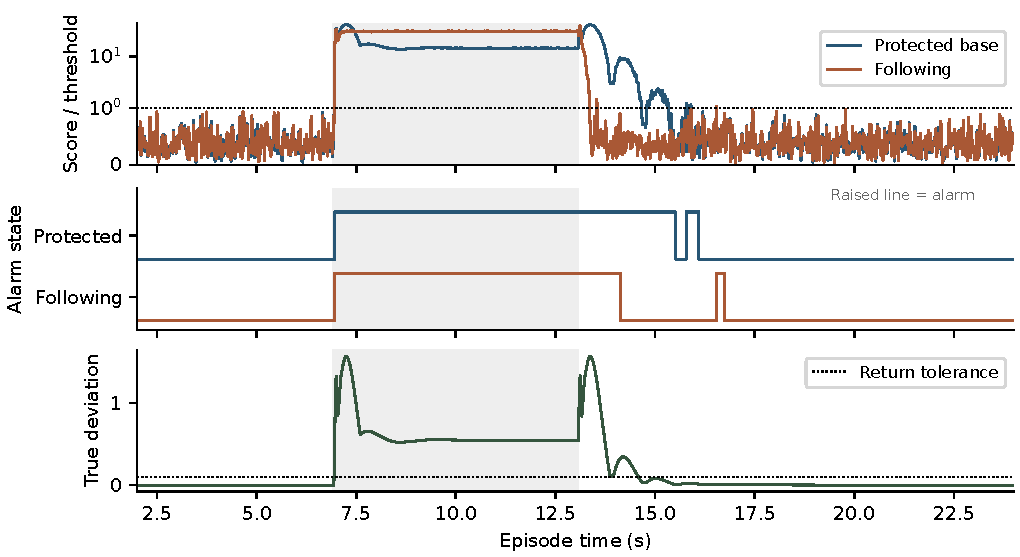
\includegraphics[width=0.77\textwidth]{figures/trace.pdf}
\caption{Post-study illustration from task N14, plant Q2, seed 17, persistent offset. Shading marks command corruption. The following residual falls while physical deviation remains above tolerance. This trace was selected to explain the aggregate contrast; it is not independent confirmatory evidence.}\label{fig:trace}
\end{figure*}

The single RBF early-clear event occurs two samples after onset, with true standardized deviation 0.01649 below tolerance 0.1. A fresh alarm starts three samples later. It is a continuity break, not an outside-tolerance clearance. A separately labelled post-study falling-edge diagnostic finds no outside-tolerance early falls for protected-reference variants, versus 108 events for following point and 82 for following dual. This clarification preserves the registered metric and failed primary decision. Persistence misses 41 events and the rolling mean misses 60; their conditional clearance fractions cannot be presented as recovery success on every event.

\subsection{Ablation and uncertainty studies}
Removing the short window changes zero alarm entries in all 189 episodes. Its contribution is unsupported under these conditions. Removing dwell reduces RBF benign points from 7,012 to 1,195, with 108 overlap hits and 108 timely clears. Its registered early-clear count remains one, on a different episode. The favorable no-dwell result is an exposed secondary finding; promoting it as a new confirmed detector would require a separately frozen study.



E1 reduces benign points from 621 to 309 using an empirical allowance, but clears only 36/108 detected events with return; its same-entry no-allowance control has 140 benign points and 108 clears. E2 reduces the harder plants' allowances by 51.27\% and 38.56\%, yet fails overall feasibility. Appendix~\ref{app:earlier} summarizes earlier findings under their distinct calibration.

E4 certifies enough normal endpoints on 20/36 constructed traces, failing its all-traces criterion. Averaging competes with temporal correlation and within-window motion. Appendix~\ref{app:uncertainty} summarizes the conditional assumptions and outcome; these are direct synthetic residuals, not attack trials.

\subsection{Matched no-dwell control and saved timing analysis}
A separately versioned replay adds the missing base no-dwell control on the already exposed E5 observations. It changes neither fitted models nor original thresholds, scores, windows or eligible support. All 3,213 original outcomes and alarm arrays replay exactly; the extension contains 3,402 outcomes. These are explanatory results, not fresh confirmation.

\begin{table*}[t]\centering\setlength{\tabcolsep}{4pt}
\caption{Matched exposed-data replay: all six selected contrasts share 89,100 benign points (0.495 h) and 108 events. Durations and delays are seconds. All overlap 108 events; ``clear'' is conditional first inactivity at/after return, not continuous retention. Gaps use the original continuity definition.}\label{tab:matchedreview}
\begin{tabular}{lrrrrrrr}\toprule
Method & Occupancy (\%) & Starts/h & Run med./p95 & Fresh & Detect med./p95 & Clear med./p95 & Gaps\\\midrule
Base point & 0.957 & 1537.4 & 0.02/0.04 & 108/108 & 0.02/0.08 & 0.08/0.78 & 38 \\
Base dual & 8.031 & 1208.1 & 0.20/0.42 & 101/108 & 0.02/0.08 & 0.92/1.07 & 2 \\
Base no dwell & 1.345 & 1537.4 & 0.02/0.06 & 108/108 & 0.02/0.08 & 0.65/0.78 & 2 \\
RBF point & 0.937 & 1501.0 & 0.02/0.04 & 108/108 & 0.02/0.09 & 0.08/0.78 & 39 \\
RBF dual & 7.870 & 1191.9 & 0.20/0.42 & 105/108 & 0.02/0.08 & 0.94/1.07 & 3 \\
RBF no dwell & 1.341 & 1501.0 & 0.02/0.06 & 108/108 & 0.02/0.09 & 0.65/0.78 & 1 \\
\bottomrule\end{tabular}

\end{table*}

Base no-dwell has 1,198 benign points against RBF's 1,195, only three points (0.25\%) apart. Both achieve 108 fresh detections and no observed alarm inactivity while physical deviation exceeds tolerance. Base point also has no such inactivity. Removing dwell lowers occupancy by 83.26\% for base and 82.96\% for RBF, but increases starts from 598 to 761 and 590 to 743 respectively. Median benign alarm duration falls from 0.20 to 0.02 s. This is a fragmentation trade-off, not evidence that RBF supplies the improvement.

\begin{figure*}[t]\centering
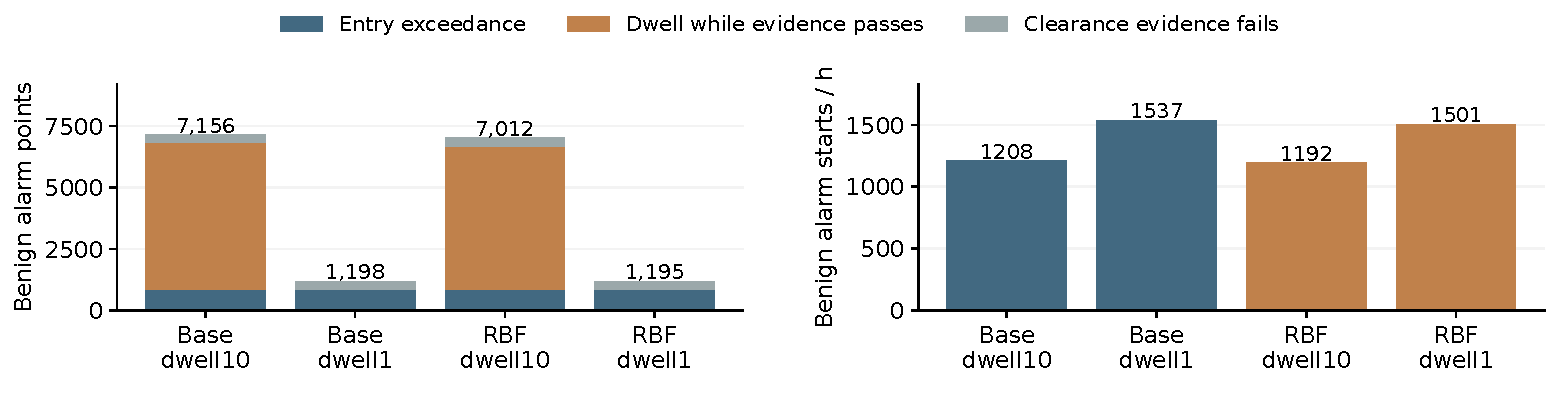
\includegraphics[width=0.92\textwidth]{figures/matched_review.pdf}
\caption{Exposed-data diagnosis. Most dual-rule benign occupancy occurs while clearance evidence already passes, because dwell retains the alarm. Removing dwell reduces occupancy but increases alarm starts. Point counts are decomposed disjointly; starts/h normalize only 0.495 pooled benign hours and do not estimate a validated deployment rate.}\label{fig:matchedreview}
\end{figure*}

For base dual, 5,958 of 7,156 benign alarm points are retained despite passing clearance evidence, compared with 853 current score exceedances and 345 points lacking clearance evidence. The corresponding RBF counts are 5,817, 835 and 360. Noise and persistence interact: noiseless reference error alone exceeds the threshold at 150 base points, whereas noisy scores exceed it at 853. The overlapping noise/reference subsets cannot be added as causal fractions. Authorized-offset boundaries contain 270/467 base exceedances within 2,700/29,700 points; unchanged operation has only 19/188 at the same clock windows. Transients matter, but do not explain most retained occupancy.

Appendix~\ref{app:earlier} reports timing and strata. RBF no-dwell worsens Q1 and tasks N14/O14; pooled improvement is not uniform. No-dwell median clearance is 0.65 s for both references, versus 0.92/0.94 s with dwell. Following point has zero median clearance because 105/108 alarms are already inactive at physical return, yet loses 6,984 outside-tolerance points after detection. Persistence and rolling mean have 41 and 60 misses; their conditional delays exclude those misses. CUSUM has 108 observed returns and 108 censored clearances. These distributions explain why a nominal 108/108 inactive-by-return fraction cannot establish successful recovery monitoring.

\subsection{Fresh contextual-envelope evaluation}\label{sec:contextresults}
Normal-only selection chooses memory 40; both memories produce zero alarms on the 29,700 M13 development points, and the lower mean width breaks the tie. Each plant uses 9,900 training and 9,900 calibration points. The selected context cutpoints and three widths are Q1 $(0.06969,0.45982)$ and $(0.03599,0.03817,0.04685)$; Q2 $(0.06916,0.45650)$ and $(0.03584,0.04389,0.08261)$; Q3 $(0.06924,0.45714)$ and $(0.05273,0.06456,0.12401)$. Every bin contains at least 102 calibration points, so fallback is unused. Q3's high-context width exceeds tolerance 0.1; the candidate cannot clear in that bin even at zero residual.

All 216 episodes and 2,376 method--episode outcomes complete. Table~\ref{tab:contextfinal} retains all eleven methods. The contextual interval reduces benign points from 42,193 to 332 (99.21\%) and starts from 3,341 to 94 (97.19\%) relative to base dual. Fresh detections rise from 136 to 144. Nevertheless, \textbf{the prospective composite criterion fails}: fresh-detection p95 is 0.731 s versus 0.040 s, exceeding the allowed 0.2 s increase; outside-tolerance inactivity rises from zero to 679/66,357 points (1.023\%); and the joint event count falls from 144 to 62. These three failed cost constraints cannot be replaced by the favorable occupancy result.

\begin{table*}[t]\centering\setlength{\tabcolsep}{4pt}
\caption{Complete fresh synthetic campaign: 72 benign episodes, 424,800 eligible benign points (2.36 h) and 144 attack events. Every method overlaps 144 events, has an observed physical return and is inactive by return + 5 s. Fresh and joint counts use 144; outside inactivity includes detection delay, over 66,357 above-tolerance points. Delays are seconds.}\label{tab:contextfinal}
\begin{tabular}{lrrrrrrrr}\toprule
Method & Benign (\%) & Starts/h & Fresh & Fresh p95 & Outside inactive & Joint & Clear med./p95 & F1\\\midrule
Base dual & 9.932 & 1415.7 & 136 & 0.040 & 0 & 144 & 0.92/1.06 & 0.566 \\
Base no dwell & 1.560 & 2093.6 & 144 & 0.040 & 1 & 143 & 0.59/0.76 & 0.805 \\
RBF dual & 10.156 & 1439.0 & 136 & 0.040 & 0 & 144 & 0.92/1.08 & 0.561 \\
RBF no dwell & 1.620 & 2137.7 & 144 & 0.040 & 1 & 143 & 0.60/0.76 & 0.802 \\
Following point & 1.202 & 1844.9 & 144 & 0.040 & 8,124 & 0 & 0.00/0.00 & 0.902 \\
Tolerance point & 0.104 & 100.8 & 144 & 0.197 & 284 & 40 & 0.00/0.02 & 0.891 \\
Three-of-five & 0.504 & 133.9 & 144 & 0.080 & 256 & 12 & 0.14/0.78 & 0.852 \\
Global interval & 0.072 & 45.8 & 144 & 0.777 & 767 & 62 & 0.06/0.12 & 0.885 \\
Context point & 0.035 & 44.5 & 144 & 0.731 & 1,831 & 0 & 0.00/0.00 & 0.899 \\
Context hysteresis & 0.047 & 44.5 & 144 & 0.731 & 1,016 & 12 & 0.00/0.02 & 0.894 \\
Context interval & 0.078 & 39.8 & 144 & 0.731 & 679 & 62 & 0.06/0.12 & 0.886 \\
\bottomrule\end{tabular}

\end{table*}
\begin{figure*}[t]\centering
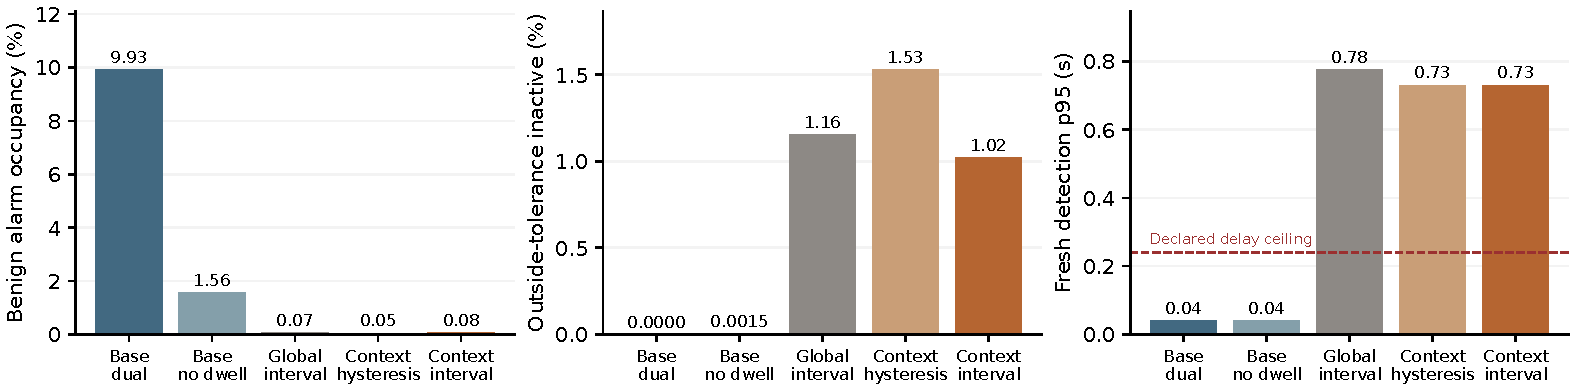
\includegraphics[width=\textwidth]{figures/context_final.pdf}
\caption{Prospectively declared trade-off on new trajectory and plant conditions. The contextual interval reduces benign burden, but increases outside-tolerance inactivity and violates the delay constraint against base dual. Its recovery rule helps relative to matched contextual hysteresis; a constant-width interval achieves the same joint event count. The full roster is retained in Table~\ref{tab:contextfinal}.}\label{fig:contextfinal}
\end{figure*}

The recovery component has a measurable effect within the contextual family: it reduces outside-tolerance inactive points from 1,016 for ordinary hysteresis to 679 and raises joint events from 12 to 62, with identical 144 fresh hits and p95 delay. This comes with 332 rather than 201 benign alarm points, although starts fall from 105 to 94. All declared matched-hysteresis constraints pass. The constant-width interval gives 305 benign points, 108 starts, 767 outside-inactive points and the same 62 joint events. Thus contextual conditioning has a mixed cost profile and does not account for a new dominant method.

Ordinary controls remain informative. The tolerance point rule has 441 benign points and 284 outside-inactive points, with p95 delay 0.197 s; the three-of-five trigger has 2,143 benign points, 256 outside-inactive points and p95 delay 0.080 s. No-dwell variants retain most event support but fragment alarms. Following point attains higher schedule $F_1$ (0.902) while losing 8,124 outside-tolerance points and yielding no joint successes. Missing detections and absent returns happen to be zero in this campaign; favorable conditional clearance still conceals different retention behavior.

A post-evaluation trace decomposition separates the remaining failures: 299 outside-tolerance inactive samples occur before first detection and 380 after it. Of the latter, 321 occur after the first ten-point physical-return interval because distance later crosses tolerance again. Across 39 events with such recrossings, the candidate is inactive on recrossings in 38. Of all 679 inactive-outside samples, 678 lie in the unresolved $L_t\le0.1<U_t$ band and one has incorrect empirical inside evidence. Retaining a previously inactive state through uncertainty is therefore distinct from observing a falling alarm edge outside tolerance. The finite return label is not permanent recovery. This descriptive diagnosis did not select a variant or change the failed criterion.

All 332 benign candidate alarm points occur during authorized changes on perturbed plants. Outside-inactive points are 335 on original plants and 344 on perturbed ones; Lissajous/smoothstep tasks contribute 218/461. The uncertainty band contains 5,636/424,800 benign points (1.327\%); no tested command context exceeds its training maximum. Neither fact validates unseen contexts.

The bounded investigation therefore establishes an additional operating trade-off, not the required original, scientifically justified improvement. Input-dependent thresholds, interval subtraction and hysteresis already exist. Neither these results nor the previous RBF audit establish superiority over CASPER, Kaisar or a complete published robotic monitoring system. The intended contribution remains unresolved; the newly exposed conditions cannot confirm an outcome-informed redesign.


\subsection{Computational cost and verification}
E5 normal development takes 16.115 seconds wall and 15.189 seconds worker CPU, with 53.23 MiB sampled peak memory. The final audit takes 27.515 seconds wall and 26.656 seconds CPU, with 90.17 MiB sampled memory and 83.44 MiB outputs. The IMU study takes 764.794 seconds wall, 753.252 seconds CPU and 553.05 MiB sampled memory. These are whole-pipeline measurements with shared work, not isolated inference latency or real-time guarantees.

The recent forecast campaign consumes 1208.167 seconds wall and 1199.209 seconds summed worker CPU, with 521.44 MiB maximum sampled memory and 14.48 MiB monitored outputs. All nine checkpoints reproduce their saved predictions exactly. The separate five-fold diagnostic uses 0.485 seconds wall and 0.297 seconds CPU. These are pipeline costs, not isolated inference latency.

The fresh contextual campaign takes 103.197 s wall, 102.722 s CPU, 78.42 MiB sampled memory and 205.36 MiB outputs, within its frozen limits. Twelve synthetic tests, 4,107 read-back checks and a separate AI-agent arithmetic review with 29,381 checks pass. These are technical checks, not independent human replication. Normal-only resource gates initially rejected runtime/storage estimates; a cache-aware estimate and lossless compact export admitted the unchanged scientific study before final generation.

The matched replay takes 1.633 s supervised wall and 1.296 s CPU, with 74.0 MiB sampled memory. Twelve synthetic tests, 71,523 worker parity checks and 112,847 fresh-process checks pass; a monitor-denied, zero-output first attempt is preserved. No training or new simulation is involved.

The reproducibility records retain every attempt, original outcome and model/score replay check. Appendix~\ref{app:provenance} identifies the evidence packages.


\section{Conditional prediction and sustained deviation}\label{sec:conditional}
The preceding experiments motivate a more specific question: how much can a predictor use observations to correct nominal-model error before that correction also weakens evidence of an unauthorized trajectory? A separate execution of RAPT~\cite{rapt} examines this issue. It is a transferred detector-core experiment, not a reproduction of the original humanoid study or a test of a claimed recovery guarantee.

\subsection{A fixed detector on exposed simulations}
The released model uses a residual encoder, a gated recurrent unit and Gaussian mean/variance outputs. We retain the author architecture and training loop, with batch size 32, one CPU thread and 100 epochs. Nine Q1 episodes from task K13 provide training; nine M13 episodes select the checkpoint by normal-development negative log likelihood; nine L13 episodes calibrate the released gates after checkpoint selection. Each population contains unchanged operation and two authorized-change conditions over three noise seeds. The selected checkpoint is epoch 14. A completed epoch budget does not imply convergence: development loss deteriorates later in this run. Observations are joint positions and velocities, and inputs include protected desired motion rather than the original humanoid observation/action interface.

For the frozen exploratory replay, this single checkpoint scores all 36 already exposed Q1 episodes from the contextual campaign. It detects 9 of 24 interventions and misses 15, with 5,175 alarms among 70,800 eligible benign points (7.309\%). Both declared model-only and hybrid modes give identical decisions. The detector is inactive on 9,448 of 10,689 physically outside-tolerance points. All six persistent-offset final quarters are inactive, covering 747 outside-tolerance points. The L19 cases react initially and later become inactive; the S19 cases are already below threshold early. No mode is selected after seeing these outcomes. Earlier ARX references have different commissioning histories, so their scores do not form a matched-training superiority comparison with this RAPT run.

\subsection{Separating prediction error from predicted variance}
The released channel score is
\begin{equation}
 \ell_{t,j}=(y_{t,j}-\mu_{t,j})^2\exp(-\nu_{t,j}),
 \label{eq:raptdecomposition}
\end{equation}
where $y$ is training-standardized and $\nu$ is predicted log variance. The training objective includes a log-variance term that is absent from this released score. Both mean and variance depend on observation history. A falling score alone therefore does not identify which component changed, or why.

A further no-fit replay saves both components without changing inputs, weights or calibration. All 518,400 channel-score values over 129,600 rows match the earlier output exactly; 126,000 rows are eligible after warmup. On positive-score support,
\begin{equation}
 \overline{\log\ell}=\overline{\log(y-\mu)^2}-\overline{\nu}.
\end{equation}
First-to-last quarter differences are computed separately within each channel. All 36 episodes and all conditions are retained in the execution record; no zero squared-error or score entries were excluded from these summaries. Figure~\ref{fig:decomposition} shows the persistent-offset contrasts that motivated the diagnostic.

\begin{figure*}[t]\centering
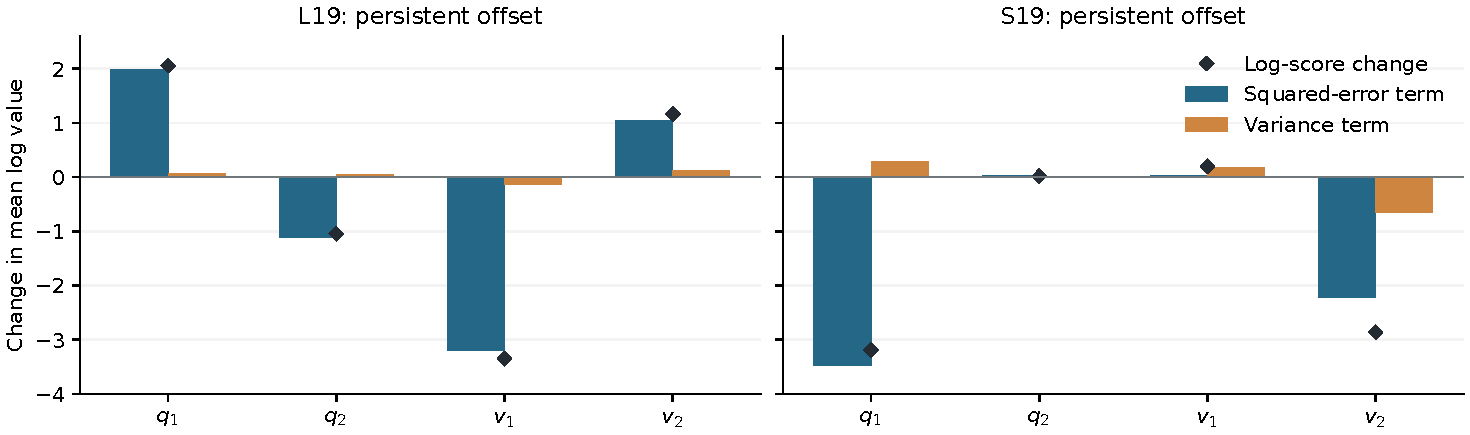
\includegraphics[width=0.91\textwidth]{figures/score_decomposition.pdf}
\caption{Exploratory decomposition of persistent-offset channel scores. Bars average each episode's last-minus-first quarter mean-log difference across three noise seeds. The numerator and negative log-variance terms add to the channel log-score change. They do not add to the max-over-gates detector risk. All position/velocity channels for both tasks are shown; the cases were already exposed before this diagnostic.}\label{fig:decomposition}
\end{figure*}

L19 position channel $q_1$ has an increasing mean log squared error ($+1.9838$), while the mean log squared error of its velocity channel $v_1$ decreases ($-3.2055$). For S19 $q_1$, the numerator decreases by $3.4826$, but decreasing variance partly opposes the score decline. These results exclude a uniform explanation based on all persistent position errors shrinking, or on variance inflation alone. They do not identify recurrence, immediate observation conditioning, phase, task transfer or calibration as the cause. Network parameters remain fixed during replay. The diagnostic adds visibility to an existing result; it supplies neither fresh attack confirmation nor evidence that a proposed replacement works.


\section{A constrained observation-correction candidate}\label{sec:gain}
We investigate whether observation correction can reduce nominal mismatch while preserving an explicit response to sustained displacement. The hypothesis concerns the useful trade-off achieved by a complete causal monitor. Protected prediction already appears in robotic security~\cite{robotactive}. Bi-Lipschitz residual separation~\cite{iresnet}, Lipschitz-autoencoder anomaly separation~\cite{lipschitzauto}, and support-conditional pointwise reconstruction-error bounds~\cite{diffint} also predate this construction. The construction below is not presented as a new theorem.

\subsection{Information and correction contract}
Let $b_t=B(u_{\leq t})$ be a normally fitted, frozen motion reference based on protected authorized commands. Fixed training scales transform all four observation channels. Define $z_t=y_t-b_t$, and let $c_t$ contain only causal protected command context. A small observation-correction model has the form
\begin{align}
 h_t&=\tanh(W_hh_{t-1}+W_zz_{t-1}+W_cc_t+d),\label{eq:gainstate}\\
 a_t&=W_oh_t,\qquad \mu_t=b_t+a_t.
\end{align}
The induced infinity norm is the maximum absolute row sum. Hard parameter constraints enforce
\begin{equation}
 \begin{aligned}
 \|W_h\|_\infty&\leq\rho<1,&\quad \|W_z\|_\infty&\leq\beta,\\
 \|W_o\|_\infty&\leq\gamma,&\quad \frac{\gamma\beta}{1-\rho}&\leq\kappa<1.
 \end{aligned}
 \label{eq:gainconstraints}
\end{equation}
The score is $R_t=\max_j |y_{t,j}-\mu_{t,j}|/s_{t,j}$, with $0<s_{t,j}\leq s_{\max}$ fixed from normal data or determined only by protected command context. Observation-conditioned scale changes would require their own analysis. The initial state, resets, timing, reference and normalization are part of the information contract; an unexamined measurement-derived phase or reset can invalidate it.

\subsection{Conditional sensitivity and its limitations}
Compare two observation streams with identical protected commands, weights, initialization and reference. Write their observation difference as $\delta_t$ and their correction difference as $\Delta a_t$. The Lipschitz property of $\tanh$ and the row-sum bounds give
\begin{equation}
 \|\Delta a_t\|_\infty\leq\gamma\beta
 \sum_{s<t}\rho^{t-1-s}\|\delta_s\|_\infty.
 \label{eq:fadingbound}
\end{equation}
For a displacement plateau of magnitude $D$, with no larger earlier displacement, this is at most $\kappa D$. If $r_t^0$ is the nominal residual, the reverse triangle inequality yields
\begin{equation}
 \|r_t^a\|_\infty\geq (1-\kappa)D-\|r_t^0\|_\infty.
 \label{eq:plateaubound}
\end{equation}
Thus a genuine nominal bound $\|r_t^0\|_\infty\leq E$ gives the sufficient strict-alarm condition
\begin{equation}
 D>\frac{E+\tau s_{\max}}{1-\kappa}\quad\Longrightarrow\quad R_t>\tau.
 \label{eq:gainradius}
\end{equation}
This argument is a direct contractive-residual calculation, related to the lower distance bound for invertible residual maps~\cite{iresnet}. It is conditional on the stated pairing and bounds. A finite development maximum is not a bound on all future nominal errors. An observed displacement is not an attack-command amplitude, and a normalized radius is not a physical safety tolerance. After a larger transient, Eq.~\eqref{eq:fadingbound}, rather than the plateau simplification, must account for its remaining history. The analysis concerns real-arithmetic maps represented by the fitted weights; numerical norm checks and finite floating-point tests do not establish a verified machine-arithmetic operational guarantee. Neither this bound nor an alarm falling edge certifies permanent recovery.

Amplitude saturation supplies another ordinary bound. If $\|a_t\|_\infty\leq C$ for both streams, then $\|\Delta a_t\|_\infty\leq2C$. The strongest of these two elementary sufficient radii is
\begin{equation}
 D_{\rm suff}=\min\!\left\{
 \frac{E+\tau s_{\max}}{1-\kappa},\,
 E+\tau s_{\max}+2C\right\},
 \label{eq:capradius}
\end{equation}
using the gain term only when $\kappa<1$. For Eq.~\eqref{eq:gainstate}, $C\leq\gamma$. A clipped linear correction can also exploit the amplitude bound; excluding it would overstate the neural construction's distinction.

\subsection{Why ordinary controls are decisive}
A command-only reference has $\kappa=0$ and the strongest displacement sensitivity, although its nominal error can be large. A leaky residual filter,
\begin{equation}
 a_t=\rho a_{t-1}+(1-\rho)\kappa z_{t-1},
\end{equation}
has the same gain budget. A multivariate finite-impulse-response correction satisfies it when the sum of its lag-matrix norms is at most $\kappa$. The nonlinear model must therefore improve nominal fit sufficiently to offset the sensitivity it spends, under the same information, reference, scale and normal-data selection. Command-context capacity and saturation also require matched controls.

The inspected 2025 recurrent fault-diagnosis preprint~\cite{renpreprint} gives an upper response-gain bound, treats the corresponding target-fault sensitivity condition as necessary, and leaves a sufficient sensitivity construction to future work. Its later journal version (doi:~\url{https://doi.org/10.1016/j.automatica.2026.113096}) has not been inspected at equation level here; the preprint's stated future work is not evidence of an open gap in that final article. More broadly, contraction and reconstruction-based anomaly separation already exist~\cite{iresnet,lipschitzauto,diffint}. Any originality claim must concern a demonstrably distinct and useful complete method beyond those results, rather than the bound, a new name or a change of application alone.


\subsection{Prospectively frozen normal feasibility test}\label{sec:gainpilot}
Before any new attack evaluation, we froze a finite normal-only comparison. The admitted data are the nine exposed Q1/K13 training episodes and nine Q1/M13 development episodes used in the recurrent-model track, each with 1,200 rows and a 100-row warmup. Each role supplies 9,900 eligible targets. L13 calibration, attacks and simulator truth are excluded. Separate observation and command means and standard deviations are fitted only on eligible K13 rows. A common command-only reference uses 16 preceding-command lags, ridge coefficient 0.001 and an unpenalized intercept. This reference is refitted under the common contract; it is not the older ARX commissioning model.

Six constrained adapters cross $\kappa\in\{0.25,0.5,0.75\}$ with $\rho\in\{0.25,0.75\}$. Each has eight hidden units and 200 stored parameters, with $\beta\leq1-\rho$ and $\gamma\leq\kappa$. Trusted context consists of the preceding normalized command and its first difference. The score scale is one for every method. All nine neural fits, including two command-only controls and an unconstrained diagnostic, use seed 17, 40 fixed full-batch Adam epochs, learning rate 0.01 and weight decay $10^{-4}$. Final-epoch weights are retained without development checkpoint selection. Training windows contain 48 burn-in rows and up to 48 scored targets; their zero initialization differs from the full-episode state used for comparative scoring. The windows preserve chronology and do not cross episodes or roles.

The 33-method roster also contains the direct reference, five-lag constrained multivariate residual FIRs, additive command-only-network plus FIR controls, leaky filters, an unconstrained FIR, clipped FIRs and four ordinary residual random-walk Kalman filters. Linear models share protected context and an intercept. The constrained FIR solver projects each output's residual coefficients across all lags onto an $\ell_1$ ball; its exact history gain is the largest such row sum. Command-only nonlinear controls have unrestricted output weights, since their output cancels under the paired comparison. Clipped controls bound only the observation-dependent component. All ten linear fits satisfy the predeclared projected-gradient convergence check.

For normal development, $E_{\rm dev}$ is the largest absolute channel residual and $\tau_{\rm dev}$ is the 99th-percentile maximum-channel score, using sorted zero-based rank 9,800 of 9,900 scores. Substitution into Eq.~\eqref{eq:capradius}, with actual fitted norm bounds, gives an \emph{empirical radius proxy}. It is a selection quantity, not a deployment certificate or independent false-alarm calibration. The candidate and strongest certified comparator are each selected by smallest radius, then RMSE, then a fixed identifier. The registered gate requires at least 5\% lower radius and 2\% lower pooled RMSE against that same comparator, no episode or condition RMSE regression above 5\%, and a lower radius with no worse RMSE than the strongest same-$\kappa$ constrained/additive FIR. Missing convergence, incomplete fits or failed execution checks also block advancement.

\begin{table*}[t]\centering\small\setlength{\tabcolsep}{7pt}
\caption{All 33 normal-development outcomes. $K$ is the actual certified history-gain bound; $C$ bounds the observation-dependent correction for the paired contrast. Radius is the smaller valid gain/cap proxy. A dash means that quantity is unavailable, not zero. All rows use the same 9,900 development targets. ``Late loss drop'' marks more than 1\% training-MSE improvement from epochs 31 to 40; it is not a global convergence test.}\label{tab:gainpilot}
\begin{tabular}{lrrrrc}\toprule
Method & Actual $K$ & Cap $C$ & Radius proxy & RMSE & Late loss drop\\\midrule
Direct reference & 0 & 0 & 3.4098 & 0.11623 & -- \\
Context r=0.25 & 0 & 0 & 3.4178 & 0.11719 & no \\
Context r=0.75 & 0 & 0 & 3.4181 & 0.11715 & no \\
Tanh k=0.25, r=0.25 & 0.25 & 0.25 & 3.6953 & 0.10337 & no \\
Tanh k=0.25, r=0.75 & 0.25 & 0.25 & 3.7866 & 0.10702 & no \\
Tanh k=0.5, r=0.25 & 0.5 & 0.5 & 4.0368 & 0.092446 & no \\
Tanh k=0.5, r=0.75 & 0.5 & 0.5 & 4.1895 & 0.098459 & no \\
Tanh k=0.75, r=0.25 & 0.75 & 0.75 & 4.3733 & 0.083709 & yes \\
Tanh k=0.75, r=0.75 & 0.75 & 0.75 & 4.6067 & 0.091073 & no \\
Unconstrained tanh & 6.3798 & 2.5871 & 6.4328 & 0.040475 & yes \\
FIR k=0.25 & 0.25 & -- & 3.7312 & 0.087017 & -- \\
FIR k=0.5 & 0.5 & -- & 4.4109 & 0.059988 & -- \\
FIR k=0.75 & 0.75 & -- & 6.4616 & 0.037311 & -- \\
Context r=0.25 + FIR k=0.25 & 0.25 & -- & 3.7318 & 0.087007 & -- \\
Context r=0.25 + FIR k=0.5 & 0.5 & -- & 4.4165 & 0.059971 & -- \\
Context r=0.25 + FIR k=0.75 & 0.75 & -- & 6.4615 & 0.03725 & -- \\
Context r=0.75 + FIR k=0.25 & 0.25 & -- & 3.7318 & 0.087007 & -- \\
Context r=0.75 + FIR k=0.5 & 0.5 & -- & 4.4169 & 0.059971 & -- \\
Context r=0.75 + FIR k=0.75 & 0.75 & -- & 6.4616 & 0.037249 & -- \\
Unconstrained FIR & 1.6938 & -- & -- & 0.026939 & -- \\
Clipped FIR C=0.25 & 1.6938 & 0.25 & 3.4167 & 0.082472 & -- \\
Clipped FIR C=0.5 & 1.6938 & 0.5 & 3.4982 & 0.069022 & -- \\
Clipped FIR C=0.75 & 1.6938 & 0.75 & 3.6375 & 0.058067 & -- \\
Leaky k=0.25, r=0.25 & 0.25 & -- & 3.8463 & 0.088432 & -- \\
Leaky k=0.25, r=0.75 & 0.25 & -- & 3.9979 & 0.091762 & -- \\
Leaky k=0.5, r=0.25 & 0.5 & -- & 4.5422 & 0.061615 & -- \\
Leaky k=0.5, r=0.75 & 0.5 & -- & 5.0827 & 0.069441 & -- \\
Leaky k=0.75, r=0.25 & 0.75 & -- & 6.7292 & 0.03791 & -- \\
Leaky k=0.75, r=0.75 & 0.75 & -- & 8.8905 & 0.052101 & -- \\
KF q/r=0.01 & 1 & -- & -- & 0.072175 & -- \\
KF q/r=0.1 & 1 & -- & -- & 0.043984 & -- \\
KF q/r=1.0 & 1 & -- & -- & 0.029287 & -- \\
KF q/r=10.0 & 1 & -- & -- & 0.025881 & -- \\
\bottomrule\end{tabular}

\end{table*}

\subsection{Outcome and interpretation}
The gate fails (Table~\ref{tab:gainpilot}). The selected adapter has $\kappa=\rho=0.25$. Its RMSE is 0.10337 versus 0.11623 for the selected direct-reference comparator, an 11.06\% reduction. Its radius proxy is nevertheless 3.69533 versus 3.40982, an 8.37\% increase rather than the required 5\% reduction. The same-budget FIR has RMSE 0.08702, better than the candidate, although its radius of 3.73124 is slightly larger. Thus both the primary radius condition and the same-budget RMSE condition fail; the episode/condition regression and implementation clauses pass.

The selected adapter's gain-only proxy is 4.26044. Its smaller reported value comes from the ordinary amplitude-cap argument. This matters because saturation is also available to a simple control. The clipped FIR with $C=0.25$ has radius 3.41671 and RMSE 0.08247, both smaller than the selected neural values. A descriptive check of the complete prespecified roster finds that this same clipped FIR dominates all six constrained neural candidates on both quantities. All six candidates obtain their tighter proxy from the amplitude cap, not the gain bound. These observations preserve the original failed criterion. Figure~\ref{fig:gainpilot} shows the radius/error trade-off and all neural training histories.

\begin{figure*}[t]\centering
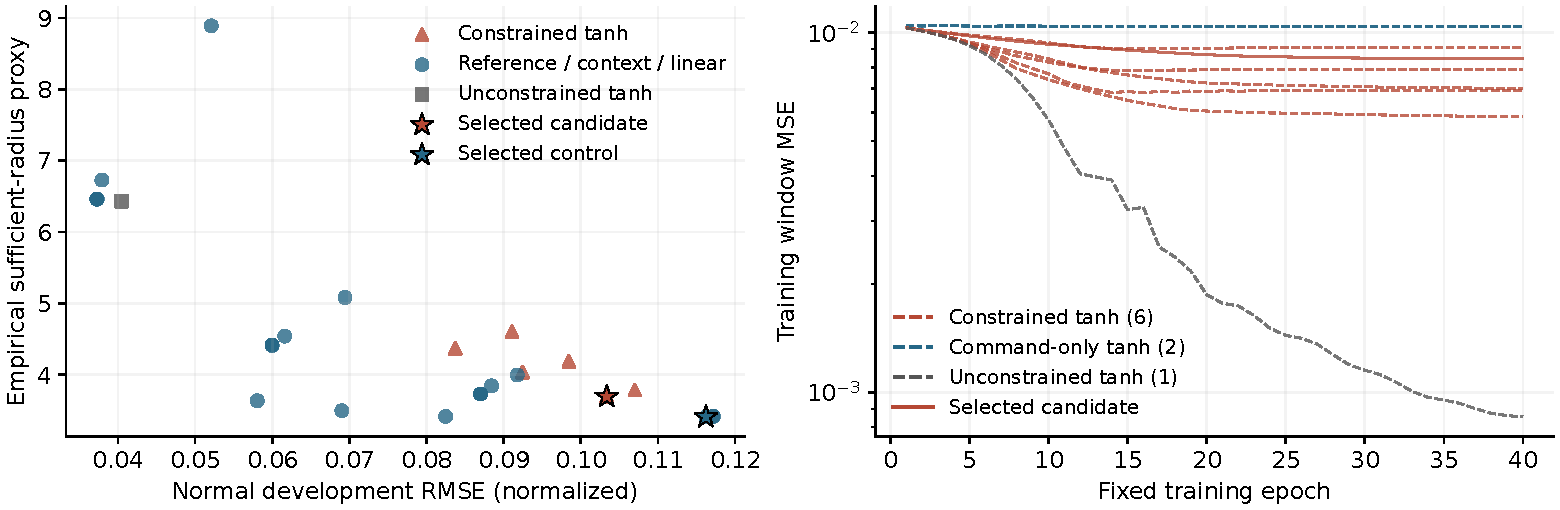
\includegraphics[width=0.94\textwidth]{figures/gain_feasibility.pdf}
\caption{Normal-only feasibility. Left: every method with a finite radius proxy; methods without one remain in Table~\ref{tab:gainpilot}. Stars mark the candidate and comparator chosen by the predeclared rule. Lower values are preferred on both axes. Right: all nine fixed 40-epoch training histories. These are exposed development and training results, without attack outcomes, confidence intervals or an operational guarantee.}\label{fig:gainpilot}
\end{figure*}

The selected adapter does not trigger the predeclared late-improvement flag. One other constrained adapter and the unconstrained neural diagnostic do. Neither flag state proves global optimization, and this finite run does not establish that every possible nonlinear model is inferior. It rejects advancement of this specified candidate under the declared criteria. No threshold calibration, fresh attack campaign, longer training or criterion revision follows the failure.

All 33 methods, nine neural fits and ten linear fits complete in one monitored run: 5.696 s wall, 4.810 CPU seconds, 292.4 MB sampled peak RSS and 23.69 MB output, within 120 s, 90 CPU seconds, 1 GiB and 50 MiB. Sixteen synthetic software tests pass before the 41-identity freeze. Reloaded weights reproduce all neural predictions exactly in PyTorch. A separate NumPy implementation differs by at most $2.39\times10^{-7}$ and independently reconstructs the norms, metrics, linear stationarity checks and failed decision without importing the model/evaluation helpers. Source/input identities, every fitted model, epoch history, normalized development record and prediction are retained. Runtime was conservatively admitted from a synthetic tensor fixture before research-data fitting; the fixture was not robot evidence. These AI-assisted checks support the execution record, not independent human replication or physical generalization.


\section{Discussion}\label{sec:discussion}
\subsection{What the comparisons establish}
The central distinction is between following measured behavior and preserving a reference to approved behavior. Protected evolution retains deviations in this simulator, but the ordinary ARX already provides that benefit. The nonlinear correction and dual-window assembly do not meet the registered improvement target. Existing identification, residual correction, averaging and hysteresis remain close prior art; combining them does not by itself establish an original detector.

Reference accuracy, entry scoring and clearance logic have different roles. The no-dwell contrast shows that persistence can dominate benign occupancy despite unchanged scores and thresholds. AP hides alarm retention; schedule F1 hides much of physical recovery. Both must be accompanied by event and clearance measures.

The constrained-correction pilot makes the prediction/sensitivity trade-off explicit. Better normal RMSE is not sufficient when the observation gain or saturation allowance enlarges the sufficient-deviation radius. The selected neural model does not improve the registered joint criterion, and a clipped linear predictor offers a stronger radius/error combination on the same development population. The finite design and preserved failure prevent a secondary prediction gain from replacing the intended contribution.

\subsection{Relationship to published systems}
CASPER and its successor motivate external-sensor prediction; existing hybrid twins and identification methods already establish modeling and correction. E3 does not reproduce their full attack detectors. The Gaussian argument is standard error spending. Kaisar et al. already couple observer agreement with recovery transitions; their accepted manuscript now permits a method-level comparison, although its final publisher version and matching implementation remain unverified. Command-conditioned thresholds and motion-error intervals also predate our study.

MVT-Flow's offline likelihood, public fault labels and ordinary setpoints do not supply an online cyber-recovery benchmark or authenticated commands. Compatible full-method reproduction remains unresolved.

\subsection{Limitations and next evidence}
Three original parameterizations and three fresh perturbations share one simplified simulator. Noise seeds repeat stochastic realizations, not independent plants or acquisitions. Missing physics, trusted initialization and honest sensing limit external validity. The residual diagnostic receives known noise/bias/motion bounds; no operational procedure for estimating all of them is validated. Normal-only IMU development and metadata-only public-data admission do not provide a real-robot recovery test.

A worthwhile distinct mechanism remains open. The new feasibility pilot uses one simulated plant, one fitted neural seed and exposed task-separated normal data. Its empirical maxima and thresholds cannot supply population guarantees; its real-arithmetic norm argument is not a verified finite-precision or physical safety certificate. Complete recent published-system comparison and independent real-robot cyber-recovery evidence remain unresolved. Every completed condition is now exposed and cannot also confirm an outcome-informed replacement.


\section{Conclusion}\label{sec:conclusion}
This investigation separates prediction accuracy, alarm entry and recovery evidence under a protected-command threat model. The original RBF correction fails its declared improvement criterion. The missing matched no-dwell control shows that most of its apparent occupancy advantage comes from persistence: base and RBF give 1,198 and 1,195 benign points under the same policy, with increased alarm fragmentation.

A bounded replacement uses frozen command-conditioned empirical residual intervals. On 216 newly frozen synthetic episodes, it sharply reduces benign burden and improves recovery support relative to matched contextual hysteresis. It nevertheless fails the prospective composite criterion against base dual because detection is slower, outside-tolerance inactivity increases and fewer events satisfy the joint requirement. The constant-width control also prevents attributing the result solely to conditioning. The observed component benefit does not establish an overall improvement under the declared constraints. Reference conditioning, interval decisions and hysteresis are established ingredients; a distinctive worthwhile contribution and compatible complete published-system comparison remain unresolved. The subsequent recurrent-detector decomposition shows mixed channel behavior and does not identify a universal absorption mechanism. A finite gain-limited correction study then improves normal prediction error but fails its sensitivity/error advancement criterion against ordinary controls. Its familiar contraction and saturation bounds do not supply theorem novelty. Future confirmation requires a substantively justified mechanism, genuinely fresh conditions after any outcome-informed redesign, and real-robot evidence before claims of industrial recovery performance.

\section*{Declarations}
\paragraph{Funding and competing interests.} No funding or competing interests were declared.
\paragraph{Data and code availability.} Versioned code, configurations, results and a reproducibility inventory are retained locally. No public repository release is claimed. Third-party data remain subject to provider terms; Appendix~\ref{app:provenance} records source identifiers and hashes. The article contains its supporting scientific sections; executable code, fitted artifacts and episode outputs require the separately prepared local reviewer package. A source/PDF archive alone is insufficient to rerun experiments.
\paragraph{AI assistance.} OpenAI Codex assisted with literature searches, code, experiment execution, analysis, writing and editing. The software checks and AI-assisted manuscript audits reported here are not independent scientific replication or human peer review.
\appendix
\section{Uncertainty and feasibility}\label{app:uncertainty}
\subsection{Conditional geometric bounds}
Let $\|v\|_s=\max_j|v_j|/s_j$, $d_t=\|x_t-x_t^0\|_s$ and $c_t=\|y_t-r_t\|_s$. If $\|x_t^0-r_t\|_s\le b_t$ and $\|n_t\|_s\le\eta_t$, the triangle and reverse triangle inequalities give
\begin{equation}
 \max(0,c_t-b_t-\eta_t)\le d_t\le c_t+b_t+\eta_t.\label{eq:bound}
\end{equation}
Scalar errors aligned in the same direction attain these extremes. For coordinate error boxes with half-widths $b_{t,j},\eta_{t,j}$, return within $\delta$ holds for every admissible pair exactly when
\begin{equation}
 \max_j\frac{|y_{t,j}-r_{t,j}|+b_{t,j}+\eta_{t,j}}{s_j}\le\delta.\label{eq:box}
\end{equation}
Each coordinate can attain the summed magnitude, proving necessity as well as sufficiency. If any $b_{t,j}+\eta_{t,j}>\delta s_j$, the condition is infeasible. E1 instead tests $c_t+b\le\delta$ with a maximum observed normal discrepancy $b$. That maximum combines model error and noise; Gaussian noise is unbounded. The tested rule is therefore an empirical heuristic, not a verified certificate. Dwell cannot repair $b>\delta$.

\subsection{Earlier window-evidence feasibility diagnostic}
The earlier E4 experiment assumes stationary zero-mean Gaussian AR(1) noise with known marginal deviations $\sigma_j$, correlations $\rho_j$, deterministic bias bounds $B_j$ and per-step deviation increments $L_j$. A window of length $m$ has mean variance
\begin{equation}
 V_{m,j}=\frac{\sigma_j^2}{m^2}\left[m+2\sum_{k=1}^{m-1}(m-k)\rho_j^k\right].
\end{equation}
Adding $B_j+L_j(m-1)/2$ and a Gaussian tail allowance to the absolute mean residual bounds the current deviation under these assumptions. Time allocation $\alpha_t=6\alpha/(\pi^2t^2)$ and a union bound over registered windows/channels give per-trace simultaneous coverage. This is standard error spending, not new confidence-sequence theory. Overlap does not invalidate the union bound, but unknown covariance and nonstationarity invalidate the specified noise argument.

E4 tests 36 direct residual traces with windows $\{1,41,201\}$, four noise/correlation settings, three small within-tolerance motion patterns and three paired seeds. All 216 outcomes are retained. Its envelope certifies at least 95\% of normal endpoints on only 20/36 traces, failing the all-traces criterion. Longer windows can lose feasibility because the within-window variation allowance dominates noise averaging. At marginal noise 0.06/correlation 0.95, no correctly specified control certifies even settled motion; a deliberately independent-noise approximation appears more permissive without the stated guarantee.

These residuals are synthetic and every true deviation is already within tolerance. The diagnostic cannot estimate unsafe-clearance risk or physical robot performance. The main contextual extension uses empirical instantaneous allowances rather than importing this supplied-parameter guarantee. Complete generator settings, proofs, all outcome rows and the originally rendered tables remain in the local reproduction records.

\section{Earlier comparisons and full final metrics}\label{app:earlier}

\subsection{E1: original recovery comparison}
E1 has 216 episodes, 13 methods and 135 interventions, including 27 with missing command context. Its calibration constrains stateful alarm occupancy on 20,900 normal points, unlike E5's point-score quantile. The 19-episode maximum band does not establish conformal coverage under task shift.
The tested uncertainty-return rule reduces benign points from 621 for nominal fixed return to 309, but is inactive by return + 5 s for only 36/108 detected events with return. Its matched no-allowance control gives 140 benign points and 108/108; removing dwell gives 20 points but still 36/108. Thus the apparently favorable occupancy does not establish improved recovery. The episode-band control gives zero benign points yet 75 early-clear events. These earlier 13-method outcomes use a different calibration and include unknown-context events, so they are not pooled with E5. The local reproducibility records preserve every original row and alarm array.

\subsection{E2: normal commissioning}
The finite grid contains ARX orders 4, 8, 16 and 32 and finite impulse response lengths 16, 32 and 64, each with ridge $10^{-7}$, $10^{-5}$ or $10^{-3}$, on three plants: 63 fits. Fitting and selection precede 81 new normal episodes. The selected orders are 8, 16 and 32 with ridge $10^{-7}$. Forced-latch probes measure normal clearance feasibility, not post-attack recovery. The hard-plant reductions in empirical allowance do not establish a probabilistic or deterministic error bound.
For Q1--Q3 the selected free-running ARX has standardized RMSE 0.00934, 0.00972 and 0.01439, versus 0.00948, 0.01020 and 0.01586 for ARX(4). Corresponding empirical allowances are 0.0553, 0.0716 and 0.1175; the last exceeds tolerance 0.1 and cannot support the tested certificate. Selected FIR allowances are 0.2322, 0.3971 and 0.4596 and all forced-latch probes fail. Treating the command directly as state is worse still (allowances 2.1344--2.2058). Full method/plant results remain in the executable records; these failures motivate the later correction study without constituting attack evidence.

\subsection{E5 timing and matched-control strata}
The original 17-method outcome matrix remains in Table~\ref{tab:audit}; the separately versioned replay adds base no-dwell. Table~\ref{tab:timingreview} reports all 18 timing summaries. Detection samples number 108 minus misses; clearance samples condition on observed return and detection. No physical return is absent in this E5 population. The CUSUM clearance distribution is empty because all 108 clearances are censored at five seconds. Physical-outside inactivity after detection is distinct from the original pre-return continuity gaps and is descriptive here.

\begin{table*}[t]\centering\setlength{\tabcolsep}{4pt}
\caption{Exposed E5 timing, all methods. Values are seconds; med./p95 are conditional delay summaries. Already off counts alarms inactive at physical return. Outside inactive counts samples above tolerance after detection; each sample is 0.02 s. Missing detections remain in the misses column.}\label{tab:timingreview}
\begin{tabular}{lrrrrrr}\toprule
Method & Misses & Detect med./p95 & Clear med./p95 & Already off & Censored & Outside inactive\\\midrule
Base point & 0 & 0.02/0.08 & 0.08/0.78 & 2 & 0 & 0 \\
base return1 & 0 & 0.02/0.08 & 0.92/1.04 & 0 & 0 & 0 \\
base long & 0 & 0.02/0.08 & 0.92/1.07 & 0 & 0 & 0 \\
Base dual & 0 & 0.02/0.08 & 0.92/1.07 & 0 & 0 & 0 \\
linear point & 0 & 0.02/0.08 & 0.08/0.78 & 2 & 0 & 0 \\
linear dual & 0 & 0.02/0.08 & 0.92/1.07 & 0 & 0 & 0 \\
RBF point & 0 & 0.02/0.09 & 0.08/0.78 & 2 & 0 & 0 \\
rbf return1 & 0 & 0.02/0.08 & 0.92/1.04 & 0 & 0 & 0 \\
rbf long & 0 & 0.02/0.08 & 0.94/1.07 & 0 & 0 & 0 \\
RBF dual & 0 & 0.02/0.08 & 0.94/1.07 & 0 & 0 & 0 \\
RBF no dwell & 0 & 0.02/0.09 & 0.65/0.78 & 0 & 0 & 0 \\
following point & 0 & 0.02/0.08 & 0.00/0.00 & 105 & 0 & 6,984 \\
following dual & 0 & 0.02/0.08 & 0.00/0.10 & 78 & 0 & 3,310 \\
rbf following dual & 0 & 0.02/0.08 & 0.00/0.10 & 79 & 0 & 3,318 \\
persistence point & 41 & 0.02/0.04 & 0.00/0.00 & 67 & 0 & 15,957 \\
mean21 point & 60 & 0.06/0.24 & 0.00/0.00 & 48 & 0 & 11,780 \\
base cusum & 0 & 0.04/0.17 & -- & 0 & 108 & 0 \\
Base no dwell & 0 & 0.02/0.08 & 0.65/0.78 & 0 & 0 & 0 \\
\bottomrule\end{tabular}

\end{table*}
\begin{table*}[t]\centering\setlength{\tabcolsep}{4pt}
\caption{Matched base/RBF no-dwell strata (B/R). Each plant or task has 29,700 benign observations and 36 events; each attack family has 27 events and no wholly benign episode. All strata have complete overlap/fresh coverage, no absent return and no observed outside-tolerance inactivity for these two methods. Detection/clearance p95 values are seconds.}\label{tab:stratareview}
\begin{tabular}{lrrrr}\toprule
Stratum & Benign B/R & Starts/h B/R & Detect p95 B/R & Clear p95 B/R\\\midrule
Q1 & 355/381 & 1454.5/1521.2 & 0.06/0.06 & 0.77/0.77 \\
Q2 & 509/498 & 1703.0/1636.4 & 0.08/0.09 & 0.82/0.80 \\
Q3 & 334/316 & 1454.5/1345.5 & 0.12/0.12 & 0.69/0.69 \\
N14 & 234/245 & 1169.7/1254.5 & 0.09/0.10 & 0.76/0.77 \\
O14 & 308/320 & 1193.9/1260.6 & 0.11/0.11 & 0.78/0.77 \\
P14 & 656/630 & 2248.5/1987.9 & 0.03/0.04 & 0.81/0.78 \\
brief offset & -- & -- & 0.02/0.02 & 0.80/0.80 \\
persistent offset & -- & -- & 0.02/0.02 & 0.74/0.75 \\
hold & -- & -- & 0.06/0.06 & 0.76/0.75 \\
slow & -- & -- & 0.12/0.12 & 0.81/0.77 \\
\bottomrule\end{tabular}

\end{table*}

The original base/RBF dual plant differences remain Q1 2,397/2,522 benign points, Q2 2,646/2,532 and Q3 2,113/1,958. Only Q2 contains the original continuity gaps (two/three) and preexisting alarms reducing fresh hits (29/33 of 36). Every original precision/recall and episode outcome remains in the saved evidence package; the study does not treat rows or seeds as independent robot replications.

\section{Reproducibility and source identities}\label{app:provenance}
\subsection{Recorded execution and failures}
Versioned records retain inputs, configurations, commands, dependencies, code revisions, logs and every outcome. E1--E5 correspond respectively to \path{recovery_v0.8}, \path{commissioning_v0.9}, \path{casper_convergence_v0.11}, \path{return_bound_v0.12}, and \path{residual_twin_v0.13} followed by \path{attack_audit_v0.14}. Their calibration policies are not interchangeable. The later five-fold diagnostic and author-code forecast study have separate frozen records; E1--E5 are unchanged.

The records preserve an initial monitoring-denied E1 launch and an E2 reporting-key failure repaired without changing fits. E5 has no failed scientific attempt. Its final limits were 120 s wall, 90 s CPU, 1 GiB monitored memory and 128 MiB output; sampled memory is not an instantaneous hard bound. Exact commands, costs, failures and dependencies remain in the local evidence inventory.

Original and new freeze/result manifests are bound in the local reviewer package. Asset receipts bind figures and tables to saved results. Identifiers establish provenance, not validity. Raw data and third-party manuscripts are excluded from the editable archive.

The added \path{fivefold_v0.16} diagnostic preserves its monitor-denied attempt and separately bound, scientifically unchanged repair. The \path{forecast_baselines_v0.17} study was approved for 1,800 seconds wall, 1,440 seconds CPU, 1 GiB sampled memory and 150 MiB output. All nine fresh fits stopped by CPU admission; no scientific retry or post-pilot configuration change occurred. ModernTCN, iTransformer and TimeMixer revisions are \path{56a9a2c018385}, \path{c2426e68ca13} and \path{e24610583b36}; licenses are MIT, MIT and Apache-2.0. Full identities, dependencies, hardware and commands remain in the execution records.

\subsection{Real-data identity and comparator admission}
The author-linked CASPER-1-and-2 provider-v2 nominal IMU file has SHA-256 \path{1221df9be80c229969f3f21f820837e68ad28f4ccb3949bf4013f00d6d69d62c}. Its original-paper run and clock correspondence remain unresolved.

The original voraus-AD file is linked by \url{https://github.com/vorausrobotik/voraus-ad-dataset}. It has 1,115,942,833 bytes and SHA-256 \path{c90ab1c78af52651b954d41787f7e89d750f0a128b57600b0e5ceec22621f704}. Data are CC BY-NC-SA 4.0; code is MIT. Metadata verify 2,321,690 rows, 137 columns and the 2,122 executions in Table~\ref{tab:data}. Setting 72 (PRE\_A) supplies all 948 training executions. Within-execution time resets to zero, increases strictly with increments 0.00845194--0.01211095 s, and does not establish absolute acquisition order. Maximum train/test lengths are both 1,164 rows. Process signals remain unopened.

Pinned MVT-Flow code \path{a91a86a642d23df58833b792a53de01edfd81abe} uses $\|z\|^2-\log|J|$ for training, whereas the paper/scoring use $\tfrac12\|z\|^2-\log|J|$. The paper describes three convolutions; the released default constructs two. A padding truncation is overwritten, but no test execution in this release exceeds the training length. Test AUROC is computed each epoch, while the saved checkpoint is the fixed final epoch. These discrepancies remain unresolved; they do not establish test-based selection or invalid published results.

FactoryNet v5 remains an unexecuted, partially audited preprint lead; no observations were downloaded.

\subsection{Observation-correction extension}
The added records are \path{rapt_protocol_v0.21}, its exploratory replay, \path{novelty_v0.22/decomposition}, and \path{gain_limited_v0.23}. RAPT author code is pinned at \path{d745668ffdb0e26877b1de4c9b2126af7bda5b03} under BSD-3-Clause; the executed model is a detector-core transfer with a different input/task protocol. The complete 36-episode decomposition preserves every earlier channel score exactly. Its access record permits only measurements, protected commands, validity and saved scores; the schedule is read from the previously frozen configuration.

The gain-limited pilot uses independent implementations of the stated ordinary models and constrained adapter, without executing other authors' diagnostic code. Its 41 frozen identities bind 18 normal files, source, configuration, tests, review and runtime admission. All 33 method outputs, nine fixed-epoch neural models and ten fitted linear models are retained. The criterion fails without a new attack test or post-outcome retraining. A project-local Python 3.12.15 compatibility bridge reads the existing project packages after an older interpreter symlink became unavailable; it is not an independently installed portable environment. NumPy 1.26.4 and PyTorch 2.5.1 are recorded. The score-decomposition preparation preserves a sandbox shared-memory test failure; the completed decomposition and gain-limited scientific runs each execute once under monitoring.

\begingroup\raggedright\fontsize{9.6}{10}\selectfont
\begin{thebibliography}{28}
\setlength{\itemsep}{0pt}\setlength{\parsep}{0pt}

\bibitem{securitysurvey} Abdul Rehman Qureshi, Adrián Asensio, Muhammad Imran, Jordi Garcia, Xavi Masip-Bruin. {A survey on security enhancing Digital Twins: Models, applications and tools}. \emph{Computer Communications, 238:108158}, 2025. Article 108158. \url{https://doi.org/10.1016/j.comcom.2025.108158}.

\bibitem{lifecycle} Taru Itäpelto, Mohammed Elhajj, Marten van Sinderen. {Digital twin application in lifecycle security of critical infrastructures: A systematic literature review}. \emph{International Journal of Critical Infrastructure Protection, 50:100783}, 2025. Article 100783. \url{https://doi.org/10.1016/j.ijcip.2025.100783}.

\bibitem{casper} Hakan Kayan, Ryan Heartfield, Omer Rana, Pete Burnap, Charith Perera. {CASPER: Context-Aware IoT Anomaly Detection System for Industrial Robotic Arms}. \emph{ACM Transactions on Internet of Things, 5(3):1--36}, 2024. Article 18. \url{https://doi.org/10.1145/3670414}.

\bibitem{edge} Hakan Kayan, Ryan Heartfield, Omer Rana, Pete Burnap, Charith Perera. {Real-Time Anomaly Detection for Industrial Robotic Arms Using Edge Computing}. \emph{IEEE Internet of Things Journal, 12(15):29696--29712}, 2025. \url{https://doi.org/10.1109/JIOT.2025.3569780}.

\bibitem{hybrid} Samuel Ayankoso, Eric Kaigom, Hassna Louadah, Hamidreza Faham, Fengshou Gu, Andrew Ball. {A Hybrid Digital Twin Scheme for the Condition Monitoring of Industrial Collaborative Robots}. \emph{Procedia Computer Science, 232:1099--1108}, 2024. \url{https://doi.org/10.1016/j.procs.2024.01.108}.

\bibitem{arp} Daniel Arp, Erwin Quiring, Feargus Pendlebury, et al. {Pitfalls in Machine Learning for Computer Security}. \emph{Communications of the ACM, 67(11):104--112}, 2024. \url{https://doi.org/10.1145/3643456}.

\bibitem{calibration} Tinghui Chen, Weiyi Yang, Shuai Li, Xin Luo. {Data-Driven Calibration of Industrial Robots: A Comprehensive Survey}. \emph{IEEE/CAA Journal of Automatica Sinica, 12(8):1544--1567}, 2025. \url{https://doi.org/10.1109/jas.2025.125237}.

\bibitem{identification} Koen Classens, Rodrigo A. Gonz{\'a}lez, Tom Oomen. {Recursive identification of structured systems: An instrumental-variable approach applied to mechanical systems}. \emph{European Journal of Control, 84:101238}, 2025. \url{https://doi.org/10.1016/j.ejcon.2025.101238}.

\bibitem{voraus} Jan Thieß Brockmann, Marco Rudolph, Bodo Rosenhahn, Bastian Wandt. {The voraus-AD Dataset for Anomaly Detection in Robot Applications}. \emph{IEEE Transactions on Robotics, 40:438--451}, 2024. \url{https://doi.org/10.1109/tro.2023.3332224}.

\bibitem{factory} Jonas Petersen, Pratik Jawahar, Riccardo Maggioni, et al. {FactoryNet: A Large-Scale Dataset toward Industrial Time-Series Foundation Models}. \emph{arXiv preprint}, 2026. Preprint, version 5, 8 October 2026; arXiv:2605.09081. \url{https://arxiv.org/abs/2605.09081v5}.

\bibitem{moderntcn} Donghao Luo, Xue Wang. {ModernTCN: A Modern Pure Convolution Structure for General Time Series Analysis}. \emph{International Conference on Learning Representations}, 2024. \url{https://openreview.net/forum?id=vpJMJerXHU}.

\bibitem{itransformer} Yong Liu, Tengge Hu, Haoran Zhang, et al. {iTransformer: Inverted Transformers Are Effective for Time Series Forecasting}. \emph{International Conference on Learning Representations}, 2024. \url{https://openreview.net/forum?id=JePfAI8fah}.

\bibitem{timemixer} Shiyu Wang, Haixu Wu, Xiaoming Shi, et al. {TimeMixer: Decomposable Multiscale Mixing for Time Series Forecasting}. \emph{International Conference on Learning Representations}, 2024. \url{https://openreview.net/forum?id=7oLshfEIC2}.

\bibitem{interval} Jordi Meseguer, Vicen{\c c} Puig, Teresa Escobet, Jordi Saludes. {Observer gain effect in linear interval observer-based fault detection}. \emph{Journal of Process Control, 20(8):944--956}, 2010. \url{https://doi.org/10.1016/j.jprocont.2010.06.017}.

\bibitem{fail} Chen Xu, Tony Khuong Nguyen, Emma Dixon, et al. {Can We Detect Failures Without Failure Data? Uncertainty-Aware Runtime Failure Detection for Imitation Learning Policies}. \emph{Robotics: Science and Systems XXI}, 2025. \url{https://doi.org/10.15607/RSS.2025.XXI.073}.

\bibitem{howard} Steven R. Howard, Aaditya Ramdas, Jon McAuliffe, Jasjeet Sekhon. {Time-uniform, nonparametric, nonasymptotic confidence sequences}. \emph{The Annals of Statistics, 49(2):1055--1080}, 2021. \url{https://doi.org/10.1214/20-AOS1991}.

\bibitem{kaisar} H. Kaisar, M. Rehan, I. Ahmed, M. Bilal, M. Khalid. {A Digital Twin-Based Cybersecurity Architecture for FDI Anomaly Detection and Isolation in Next Generation Robotic Vehicles}. \emph{IEEE Open Journal of the Communications Society, 7:12709--12728}, 2026. \url{https://doi.org/10.1109/OJCOMS.2026.3739185}.

\bibitem{rescue} David Ahmedt-Aristizabal, Abdelwahed Khamis, Mohammad Ali Armin, Lars Petersson. {RESCUE: Is This Alarm Worth Acting On? Counterfactual Evaluation of VLA Runtime Monitors}. \emph{arXiv preprint}, 2026. Preprint, version 1, 9 October 2026; arXiv:2610.13516. \url{https://arxiv.org/abs/2610.13516v1}.

\bibitem{inputthreshold} H. P. Rotstein, R. Ingvalson, T. Keviczky, G. J. Balas. {Input-Dependent Threshold Function for an Actuator Fault Detection Filter}. \emph{IFAC Proceedings Volumes, 38(1):211--216}, 2005. \url{https://doi.org/10.3182/20050703-6-CZ-1902.01996}.

\bibitem{motionconformal} R. Schubert, M. Loba, J. S\"unnemann, T. Stolte, M. Maurer. {Conformal Prediction of Motion Control Performance for an Automated Vehicle in Presence of Actuator Degradations and Failures}. Accepted for IEEE ITSC 2024; consulted author manuscript, version 2, 29 July 2024. \url{https://arxiv.org/abs/2404.16500v2}.

\bibitem{tsbad} Qinghua Liu, John Paparrizos. {The Elephant in the Room: Towards A Reliable Time-Series Anomaly Detection Benchmark}. \emph{Advances in Neural Information Processing Systems 37, 108231--108261}, 2024. \url{https://doi.org/10.52202/079017-3437}.

\bibitem{vus} Paul Boniol, Ashwin K. Krishna, Marine Bruel, et al. {VUS: effective and efficient accuracy measures for time-series anomaly detection}. \emph{The VLDB Journal, 34(3)}, 2025. Article 32. \url{https://doi.org/10.1007/s00778-025-00907-x}.


\bibitem{rapt}
H.~Munn, B.~Tidd, P.~Bohm, M.~Gallagher, and D.~Howard,
``RAPT: Model-Predictive Out-of-Distribution Detection and Failure Diagnosis for Sim-to-Real Humanoid Deployment,''
arXiv:2602.01515v2, preprint, 21 July 2026.
\url{https://arxiv.org/abs/2602.01515v2}.

\bibitem{robotactive}
G.~Gualandi and A.~V.~Papadopoulos,
``From Passive Monitoring to Active Defence: Resilient Control of Manipulators Under Cyberattacks,''
arXiv:2603.13003v2, 26 May 2026; ICRA 2026 acceptance author-reported.
\url{https://arxiv.org/abs/2603.13003v2}.

\bibitem{renpreprint}
F.~Ghanipoor, C.~Murguia, G.~Ferrari Trecate, and N.~van de Wouw,
``Data-Driven Sensor Fault Diagnosis with Proven Guarantees using Incrementally Stable Recurrent Neural Networks,''
arXiv:2504.19688v1, preprint, 28 April 2025.
\url{https://arxiv.org/abs/2504.19688v1}.

\bibitem{iresnet}
J.~Behrmann, W.~Grathwohl, R.~T.~Q.~Chen, D.~Duvenaud, and J.-H.~Jacobsen,
``Invertible Residual Networks,'' in \emph{Proc. ICML},
PMLR, vol.~97, pp.~573--582, 2019.
\url{https://proceedings.mlr.press/v97/behrmann19a.html}.

\bibitem{lipschitzauto}
Y.-g.~Kim, Y.~Kwon, H.~Chang, and M.~C.~Paik,
``Lipschitz Continuous Autoencoders in Application to Anomaly Detection,''
in \emph{Proc. AISTATS}, PMLR, vol.~108, pp.~2507--2517, 2020.
\url{https://proceedings.mlr.press/v108/kim20c.html}.

\bibitem{diffint}
L.~Diop and M.~Plantevit,
``Differentiable Interval Bottlenecks for Interpretable Anomaly Detection in Numerical Data,''
arXiv:2609.03878v1, 3 September 2026; ICDM 2026 acceptance author-reported.
\url{https://arxiv.org/abs/2609.03878v1}.

\end{thebibliography}

\endgroup
\end{document}
